
\documentclass[12pt]{article}

\usepackage[margin=1in]{geometry}
\usepackage[T1]{fontenc}
\usepackage[utf8]{inputenc}
\usepackage{amsmath}
\usepackage{graphicx}
\usepackage{float}
\usepackage{booktabs}
\usepackage{array}
\usepackage{url}
\usepackage{enumitem}
\usepackage[numbers,sort&compress]{natbib}
\usepackage[hidelinks]{hyperref}
\usepackage{lineno}

\numberwithin{equation}{section}
\setcounter{tocdepth}{2}
\setcounter{secnumdepth}{3}
\makeatletter
\setlength{\@fptop}{0pt}
\setlength{\@fpsep}{12pt plus 2pt minus 2pt}
\setlength{\@fpbot}{0pt plus 1fil}
\makeatother

\newtheorem{theorem}{Theorem}[section]
\newtheorem{proposition}[theorem]{Proposition}
\newtheorem{lemma}[theorem]{Lemma}
\newtheorem{corollary}[theorem]{Corollary}
\newtheorem{conjecture}[theorem]{Conjecture}
\newtheorem{definition}[theorem]{Definition}
\newtheorem{experiment}[theorem]{Experiment}

\newcommand{\RVM}{\mathrm{RVM}}
\newcommand{\diff}{\mathrm{diff}}
\newcommand{\GUE}{\mathrm{GUE}}
\newcommand{\KS}{\mathrm{KS}}
\newcommand{\rms}{\mathrm{rms}}
\newcommand{\mean}{\mathrm{mean}}
\newcommand{\median}{\mathrm{median}}
\newcommand{\Poisson}{\mathrm{Poisson}}
\newcommand{\Rayleigh}{\mathrm{Rayleigh}}
\newcommand{\Wigner}{\mathrm{Wigner}}
\newcommand{\noise}{\mathrm{noise}}

\title{A Logarithmic Phase-Walk Observable for Riemann Zeta Zeros and Riemann--von Mangoldt Backgrounds}
\author{V\'ictor Casa\~na-Giner\\
\small Faculty of Sciences, Universidad Nacional de Educaci\'on a Distancia (UNED), Madrid, Spain\\
\small Correspondence: \texttt{vcasana1@alumno.uned.es}}
\date{}

\begin{document}
\maketitle

\begin{abstract}
We introduce a logarithmic phase-walk observable for the ordinates of the nontrivial zeros of the Riemann zeta function. The construction preserves the natural order of the zero sequence and applies an exponential phase weight depending on the index. The smooth comparison sequence is obtained by Lambert \(W\) inversion of the mean Riemann--von Mangoldt zero-counting law, giving the Riemann--von Mangoldt background (RVM). The transform separates the smooth counting trend from the arithmetic phase fluctuations of the true zeta zeros. The principal observation is that the transformed zeta--RVM residual has an isotropic complex increment geometry in the Re/Im audit, for which Rayleigh is the natural planar modulus benchmark. This behaviour occurs at a different statistical level from the Montgomery--Odlyzko GUE law: GUE describes spacings of zero ordinates, whereas the Rayleigh comparison is applied to moduli of complex residual increments after the logarithmic phase-walk transform. The paper reports this planar Rayleigh behaviour as a newly detected statistical feature of zeta-zero residuals under the transform. The same observable also distinguishes the confined RVM control from the coherent finite-window morphology of the true zeta sequence.
\end{abstract}

\noindent\textbf{Keywords:} Riemann zeta function; Riemann--von Mangoldt formula; Lambert \(W\); zeta zeros; spectral statistics; quantum chaos; exponential sums; window amplitudes; GUE.\\[0.2cm]
\noindent\textbf{MSC 2020:} 11M06; 11M26; 11Y35; 81Q50; 65C05.

\linenumbers
\section{Introduction}
\label{sec:introduction}

The Riemann zeta function and its nontrivial zeros are central objects in analytic number theory.  Throughout the paper, zeros are indexed in the upper half-plane.  We write a nontrivial zero as
\begin{equation}
\rho_k=\sigma_k+i\gamma_k,
\label{eq:introduction_zero_definition}
\end{equation}
with \(0<\gamma_1\leq\gamma_2\leq\cdots\), counted with multiplicity.  Thus a repeated zero would occupy repeated consecutive indices.  If distinct zeros shared the same ordinate, an arbitrary fixed ordering within that ordinate level would give the same ordinate sequence used by the phase-walk observable.  The numerical phase-walk studied here uses tabulated critical-line ordinates and evaluates the transform on the critical line, so that the real coordinate is fixed at \(1/2\).  For the true sequence and the smooth comparison background, respectively, we use the spectral notation
\begin{equation}
E_k=\gamma_k,
\qquad
E_k^{(0)}=\gamma_k^{\RVM}.
\label{eq:introduction_energy_identification}
\end{equation}

The connection between zeta zeros and spectral statistics is one of the most important bridges between number theory and mathematical physics.  Montgomery's pair-correlation theorem predicts that, after local unfolding, the two-point correlations of high zeta zeros follow the same sine-kernel law as the bulk eigenvalues of large Gaussian Unitary Ensemble (GUE) matrices.  In unfolded units, the GUE two-point cluster kernel is
\begin{equation}
K_{\GUE}(x,y)
=
\frac{\sin \pi(x-y)}{\pi(x-y)},
\label{eq:introduction_gue_sine_kernel}
\end{equation}
and the corresponding pair-correlation density is governed by
\begin{equation}
1-\left(\frac{\sin \pi u}{\pi u}\right)^2.
\label{eq:introduction_montgomery_pair_density}
\end{equation}
The historical point is important: Dyson recognized Montgomery's formula as the GUE pair-correlation law, and Odlyzko's large-scale computations supplied striking numerical confirmation \cite{Montgomery1973,Odlyzko1987,Mehta2004}.  This is also why zeta zeros became central in the quantum-chaos analogy.  Eigenvalues of quantum Hamiltonians come from self-adjoint operators, and their finite-dimensional models are Hermitian matrices with real spectra; the GUE describes the local statistics expected for chaotic systems without time-reversal symmetry.  The Hilbert--Polya viewpoint asks, at a deeper level, whether the ordinates of zeta zeros arise from a self-adjoint spectral problem.  Random-matrix and quantum-chaotic connections were developed further by Berry, Bohigas--Giannoni--Schmit, Katz--Sarnak, Rudnick--Sarnak, Keating--Snaith, and Conrey--Snaith \cite{Berry1986,BohigasGiannoniSchmit1984,KatzSarnak1999,RudnickSarnak1996,KeatingSnaith2000,ConreySnaith2008}.  Classical work on gaps between zeta zeros provides additional spacing-level context \cite{ConreyGhoshGoldstonGonekHeathBrown1985,Soundararajan1996}.

These established statistics are spacing, correlation, or trace statistics.  The classical locally unfolded gap has the form
\begin{equation}
s_k^{\rm cl}
=
\frac{\gamma_{k+1}-\gamma_k}{\langle \gamma_{k+1}-\gamma_k\rangle_{\rm loc}},
\label{eq:introduction_classical_unfolded_gap}
\end{equation}
and therefore measures nearest-neighbor spacings after removing the local density.  This is different from testing an ordered nonlinear phase field.  Several other established constructions attach kernels or phase weights to the zeros: explicit-formula kernels convert sums over zeros into prime-power terms; Landau, Weil, and Gonek-type formulae involve sums of the schematic form \(\sum_\rho \Phi(\rho)\), \(\sum_\rho x^\rho/\rho\), or Fourier transforms of the zero measure \cite{Titchmarsh1986,Edwards1974,IwaniecKowalski2004,Landau1911,Weil1952,Gonek1993}; hybrid Euler--Hadamard models use related zero products and kernels \cite{GonekHughesKeating2007}; trace-type quantum-chaos expressions use sums such as \(\sum_\gamma e^{it\gamma}\) with a common time parameter \(t\); and fractional-part statistics such as \(\{\alpha\gamma_n\}\) form another distributional line \cite{FordZaharescu2009}.  None of these is an ordered cumulative transform with an index-dependent logarithmic clock and an RVM-subtracted complex residual.

The full Riemann--von Mangoldt counting formula has the form
\begin{equation}
N(T)
=
\frac{T}{2\pi}\log\frac{T}{2\pi}
-
\frac{T}{2\pi}
+
\frac{7}{8}
+
S(T)
+
O(T^{-1}),
\label{eq:introduction_full_rvm_count}
\end{equation}
where \(S(T)=\pi^{-1}\arg\zeta(1/2+iT)\) records the oscillatory part of the zero-counting function.  The smooth comparison used in this article is obtained by dropping \(S(T)\) and the \(O(T^{-1})\) term and inverting the mean counting law
\begin{equation}
N_0(T)
=
\frac{T}{2\pi}\log\frac{T}{2\pi}
-
\frac{T}{2\pi}
+
\frac{7}{8}.
\label{eq:introduction_mean_rvm_count}
\end{equation}
Solving \(N_0(T)=k\) gives the Lambert \(W\)-based background ordinate
\begin{equation}
\gamma_k^{\RVM}
=
2\pi
\frac{k-\frac{7}{8}}
{W\!\left((k-\frac{7}{8})/e\right)},
\label{eq:introduction_lambert_rvm_inverse}
\end{equation}
where \(W\) is the principal real branch of the Lambert function, defined by
\begin{equation}
W(x)e^{W(x)}=x.
\label{eq:introduction_lambert_w_definition}
\end{equation}
Throughout the paper, RVM means the sequence \(\{\gamma_k^{\RVM}\}\) defined by \eqref{eq:introduction_mean_rvm_count}--\eqref{eq:introduction_lambert_w_definition}.

The present paper studies such an ordered projection.  Define the logarithmic phase weight
\begin{equation}
\tau_k=\pi\frac{\log\log k}{\log k},\qquad k\geq 3,
\label{eq:introduction_proper_time}
\end{equation}
and form
\begin{equation}
z_k^\zeta=\exp\left(\frac{\tau_k}{2}+iE_k\tau_k\right).
\label{eq:introduction_transformed_term}
\end{equation}
The ordered phase-walk amplitude is
\begin{equation}
S_N^\zeta=\sum_{k=3}^{N}z_k^\zeta.
\label{eq:introduction_primary_sum}
\end{equation}
The word ordered is essential: the observable is not the unordered cloud of points \(z_k^\zeta\), but the cumulative interference generated by the zero sequence in its natural order.

The smooth comparison ordinates are those of the RVM sequence defined in \eqref{eq:introduction_lambert_rvm_inverse}.
The observable introduced here differs from the standard spacing, zero-kernel, fractional-part, and trace contexts in four structural respects: it is indexed in the natural zero order, its phase uses the scale-dependent clock \(\tau_k=\pi\log\log k/\log k\), its main object is the transformed zeta--RVM residual, and its Rayleigh comparison concerns the planar modulus of complex residual increments rather than unfolded zero spacings.  To the author's knowledge, the cited literatures do not report a Rayleigh-type planar modulus comparison for an ordered complex residual transform of zeta zeros, nor do they use an RVM-subtracted logarithmic phase-walk observable of the form studied below.

The aim of the article is to isolate structural information in the difference between the zeta-zero sequence and its RVM background.  The RVM sequence is the natural smooth asymptotic background supplied by the mean counting law \eqref{eq:introduction_mean_rvm_count}, and the arithmetic content of the zeta zeros must therefore be expressed in the way the true sequence departs from this RVM background.  The logarithmic phase-walk transform is introduced to expose this departure as a complex ordered signal rather than as a scalar error sequence.  In this sense, the observable is designed to detect geometric information in the zeta--RVM residual that is invisible to standard spacing, pair-correlation, zero-kernel, and trace statistics.  The resulting phase geometry gives a new structural characterization of zeta zeros relative to RVM, while remaining consistent with the usual GUE local-spacing picture and the RVM counting asymptotics.

\section{Materials and methods}
\label{sec:materials_methods}

\subsection{Logarithmic phase-walk observable}
\label{sec:logarithmic_proper_time_transform}

\begin{definition}
\label{def:logarithmic_proper_time}
For \(k\geq 3\), define the logarithmic proper time
\begin{equation}
\tau_k
=
\pi\frac{\log\log k}{\log k}.
\label{eq:def_logarithmic_proper_time}
\end{equation}
The lower bound \(k\geq 3\) is only a domain convention: it ensures that \(\log\log k\) is real and positive. It has no independent spectral meaning.
\end{definition}

\begin{definition}
\label{def:zeta_transform}
Let \(E_k=\gamma_k\), and let \(\sigma\) be a real amplitude parameter.  The zeta logarithmic phase-walk term is
\begin{equation}
z_k^\zeta(\sigma)
=
\exp\left(
\left(\sigma+iE_k\right)\tau_k
\right).
\label{eq:def_zeta_transform_sigma}
\end{equation}
The finite computations in this article use
\begin{equation}
z_k^\zeta
=
z_k^\zeta\left(\frac{1}{2}\right)
=
e^{\tau_k/2}e^{iE_k\tau_k}.
\label{eq:def_zeta_transform}
\end{equation}
\end{definition}

\begin{definition}
\label{def:rvm_transform}
Let \(E_k^{(0)}=\gamma_k^{\RVM}\) denote the Lambert-based RVM background ordinate.  For a real amplitude parameter \(\sigma\), the background term is
\begin{equation}
z_k^{\RVM}(\sigma)
=
\exp\left(
\left(\sigma+iE_k^{(0)}\right)\tau_k
\right).
\label{eq:def_rvm_transform_sigma}
\end{equation}
The finite computations in this article use
\begin{equation}
z_k^{\RVM}
=
z_k^{\RVM}\left(\frac{1}{2}\right).
\label{eq:def_rvm_transform}
\end{equation}
\end{definition}

\begin{definition}
\label{def:residual_term}
The residual transformed term is
\begin{equation}
d_k
=
z_k^\zeta-z_k^{\RVM}.
\label{eq:def_residual_term}
\end{equation}
\end{definition}

\begin{definition}
\label{def:cumulative_amplitudes}
The cumulative amplitudes are
\begin{align}
S_N^\zeta
&=
\sum_{k=3}^{N}z_k^\zeta,
\label{eq:def_zeta_cumulative_amplitude}
\\
S_N^{\RVM}
&=
\sum_{k=3}^{N}z_k^{\RVM},
\label{eq:def_rvm_cumulative_amplitude}
\\
S_N^{\diff}
&=
\sum_{k=3}^{N}d_k.
\label{eq:def_diff_cumulative_amplitude}
\end{align}
\end{definition}


\noindent By the definition of \(d_k\), the finite cumulative sums satisfy the algebraic decomposition
\begin{equation}
S_N^\zeta
=
S_N^{\RVM}+S_N^{\diff}.
\end{equation}
This identity separates the curve under study, \(S_N^\zeta\), from its smooth diagnostic control.  RVM is used to expose which features are imposed by the logarithmic clock and which features are amplified by the true ordinates beyond the smooth background response.


\subsection{Spectral interpretation of the phase walk}
\label{sec:spectral_proper_time_interpretation}

\noindent Under the spectral identification \eqref{eq:introduction_energy_identification}, the phase of the transformed term is
\begin{equation}
\theta_k^\zeta
=
E_k\tau_k.
\label{eq:spectral_phase}
\end{equation}
Thus \eqref{eq:def_zeta_transform} may be read as a spectral amplitude evaluated in a non-uniform phase-walk gauge.  The factor \(e^{\tau_k/2}\) is a slowly varying amplitude, while the phase \(E_k\tau_k\) carries the main interference structure.


\noindent A standard spectral trace or return amplitude would use a common time variable and terms of the form \(e^{iE_kt}\).  The present observable uses the level-dependent time \(\tau_k\).  Therefore it tests ordered phase interference rather than only the distribution of spacings.


\subsection{Semiclassical background and residual phase response}
\label{sec:semiclassical_background_residual_response}

\begin{definition}
\label{def:spectral_defect}
The spectral defect relative to the RVM background is
\begin{equation}
\delta E_k
=
E_k-E_k^{(0)}.
\label{eq:def_spectral_defect}
\end{equation}
\end{definition}


\noindent The residual has the exact factorization
\begin{equation}
d_k
=
z_k^{\RVM}\left(e^{i\delta E_k\tau_k}-1\right).
\label{eq:exact_residual_phase_response}
\end{equation}
This identity isolates the relevant fluctuation \(\delta E_k\), but it is only algebraic.  The analytical question is whether the ordered sequence of these phase defects has correlations beyond a chosen null model.


\noindent If the phase defect \(\delta E_k\tau_k\) is small enough to linearize the exponential, then
\begin{equation}
e^{i\delta E_k\tau_k}-1
\approx
i\delta E_k\tau_k.
\label{eq:linearized_phase_defect}
\end{equation}
Combining \eqref{eq:linearized_phase_defect} with \eqref{eq:exact_residual_phase_response} gives
\begin{equation}
d_k
\approx
i z_k^{\RVM}\delta E_k\tau_k.
\label{eq:linear_residual_response}
\end{equation}
This gives the physical interpretation of the residual as a first-order phase response of the logarithmic phase-walk observable to the spectral defect \(\delta E_k\).


\noindent The spectral defect \(\delta E_k=E_k-E_k^{(0)}\) is not a new source of randomness.  It should be compared with the classical oscillatory term in the Riemann--von Mangoldt counting formula.  If
\begin{equation}
N(T)
=
N_0(T)+S(T)+O(T^{-1}),
\label{eq:rvM_counting_with_ST}
\end{equation}
where
\begin{equation}
S(T)
=
\frac{1}{\pi}\arg \zeta\left(\frac12+iT\right),
\end{equation}
then the smooth inverse ordinate \(E_k^{(0)}\) is defined by \(N_0(E_k^{(0)})=k\), whereas the true ordinate satisfies \(N(\gamma_k)=k\).  Linearizing \eqref{eq:rvM_counting_with_ST} gives
\begin{equation}
\delta E_k
=
\gamma_k-E_k^{(0)}
\approx
-\frac{S(E_k^{(0)})}{N_0'(E_k^{(0)})}.
\end{equation}
Since
\begin{equation}
N_0'(T)
=
\frac{1}{2\pi}\log\frac{T}{2\pi},
\end{equation}
this gives the scale relation
\begin{equation}
\delta E_k
\approx
\left(-1\right)\frac{2\pi S(E_k^{(0)})}{\log(E_k^{(0)}/2\pi)}.
\label{eq:defect_ST_scale}
\end{equation}
Thus the zeta--background ordinate defect is essentially the zero-counting fluctuation \(S(T)\), rewritten as an ordinate displacement.


\noindent Selberg's central limit theorem is mentioned here only as background for a classical fluctuation of \(\zeta(s)\), not as a theorem about the logarithmic phase-walk observable.  In its standard form it gives Gaussian behaviour for the logarithm of the zeta function on the critical line; the argument component underlying \(S(T)\) has variance of order \(\log\log T\), with normalization depending on the convention for the argument \cite{Selberg1992,Tsang1984,RadziwillSoundararajan2017}.  This comparison does not identify the geometry found in this article, and it does not predict the Rayleigh residual law or the ordered window morphology.  It only says that the scalar ordinate defect \(\delta E_k\), before applying the new transform, lies beside a classical zeta fluctuation scale.  The new object studied in this paper begins only after this defect is inserted into the ordered logarithmic phase-walk transform.  At the level of formal scale comparison, the corresponding phase defect is
\begin{equation}
\tau_k\delta E_k
\approx
\left(-1\right)\pi\frac{\log\log k}{\log k}
\frac{2\pi S(E_k^{(0)})}{\log(E_k^{(0)}/2\pi)}.
\label{eq:proper_time_phase_defect_ST}
\end{equation}
Thus the Selberg comparison only places the input defect beside a known zeta fluctuation scale.  It does not calibrate the logarithmic phase-walk kernel and does not account for the geometry detected by the observable.  The ordered logarithmic clock and the RVM subtraction define the observable tested below, and the finite block coherence observed below is a numerical property of the ordered transformed residual.


\subsection{Mathematical-physics interpretation and spectral systems}
\label{sec:physical_systems}


\noindent The logarithmic phase-walk transform treats the ordered ordinates as a spectral sequence and attaches to the \(k\)-th level its own phase clock.  This places the observable in the language of spectral interference: the central object is not a spacing histogram, but an ordered complex amplitude whose phase advances depend on both the level position and the RVM defect.  The mathematical-physics content is therefore structural: the transform compares a Weyl-type background, an ordered spectral defect, and the cumulative interference pattern generated by their phase difference.


\begin{enumerate}[label=\textup{(\roman*)}]
\item \textbf{Quantum chaotic spectra.}  The identification \(E_k=\gamma_k\) places the zeta ordinates in the same formal role as energy levels.  The BGS conjecture relates chaotic quantum spectra to random-matrix statistics \cite{BohigasGiannoniSchmit1984}; the zeta zeros enter this circle through the Montgomery--Odlyzko/Dyson connection \cite{Montgomery1973,Odlyzko1987,ConreySnaith2008}.

\item \textbf{Trace-like spectral amplitudes.}  The sum \(S_N^\zeta\) is analogous to a finite spectral phase amplitude, except that the time is \(\tau_k\) rather than a common time \(t\).  This is why the observable is closer to ordered spectral interference than to a spacing histogram.

\item \textbf{Semiclassical background plus spectral defect.}  The RVM sequence is treated as a smooth Weyl-type background.  The residual \(d_k\) is the phase response to the fluctuation \(\delta E_k\), as shown by the exact residual response identity and the linearized response formula.

\item \textbf{Scale-dependent phase clock.}  Section \ref{sec:optional_scale_clock_interpretation} rewrites \(\tau_k\) in the scale coordinate \(u=\log k\).  This shows explicitly that the observable uses a non-uniform phase clock across the spectrum; it is a mathematical parametrization of scale, not an additional physical model.
\end{enumerate}

\subsection{Data source and computational protocol}
\label{sec:numerical_protocol_limitations}


\noindent The numerical study uses the first 2,001,052 zeta-zero ordinates from Odlyzko's public zero tables, distributed in the commonly used \texttt{zeros6} data set \cite{OdlyzkoTables}.  The source file is \texttt{zeros6.gz}, a gzip-compressed text file available directly from Odlyzko's zeta-table archive \cite{OdlyzkoTables}.  In the reproducibility repository, the working file \texttt{zeross.bin} is a binary double-precision reconstruction of the Odlyzko text table used in the local workflow, historically denoted \texttt{zeros5.txt}.  The file \texttt{zLamb.bin} is not external data: it is the binary double-precision RVM sequence obtained by applying the Lambert \(W\)-based inverse mean counting law \eqref{eq:introduction_lambert_rvm_inverse} to the same index range.  The smooth comparison sequence in the computations is precisely this Lambert-based RVM background.  No private filename is part of the mathematical definition.  A reproducible implementation needs only the public zero ordinates, the construction of \texttt{zeross.bin} and \texttt{zLamb.bin}, the logarithmic clock \(\tau_k\), and the figure-generation code.  The Python computations reported here were run with Python 3.12.13 on macOS 26.3.1, build 25D771280a, with an Apple M2 processor (8 CPU cores).



\section{Results and discussion}
\label{sec:results_discussion}

\subsection{Finite cumulative geometry}
\label{sec:finite_cumulative_geometry}

\begin{figure}[htbp]
\centering
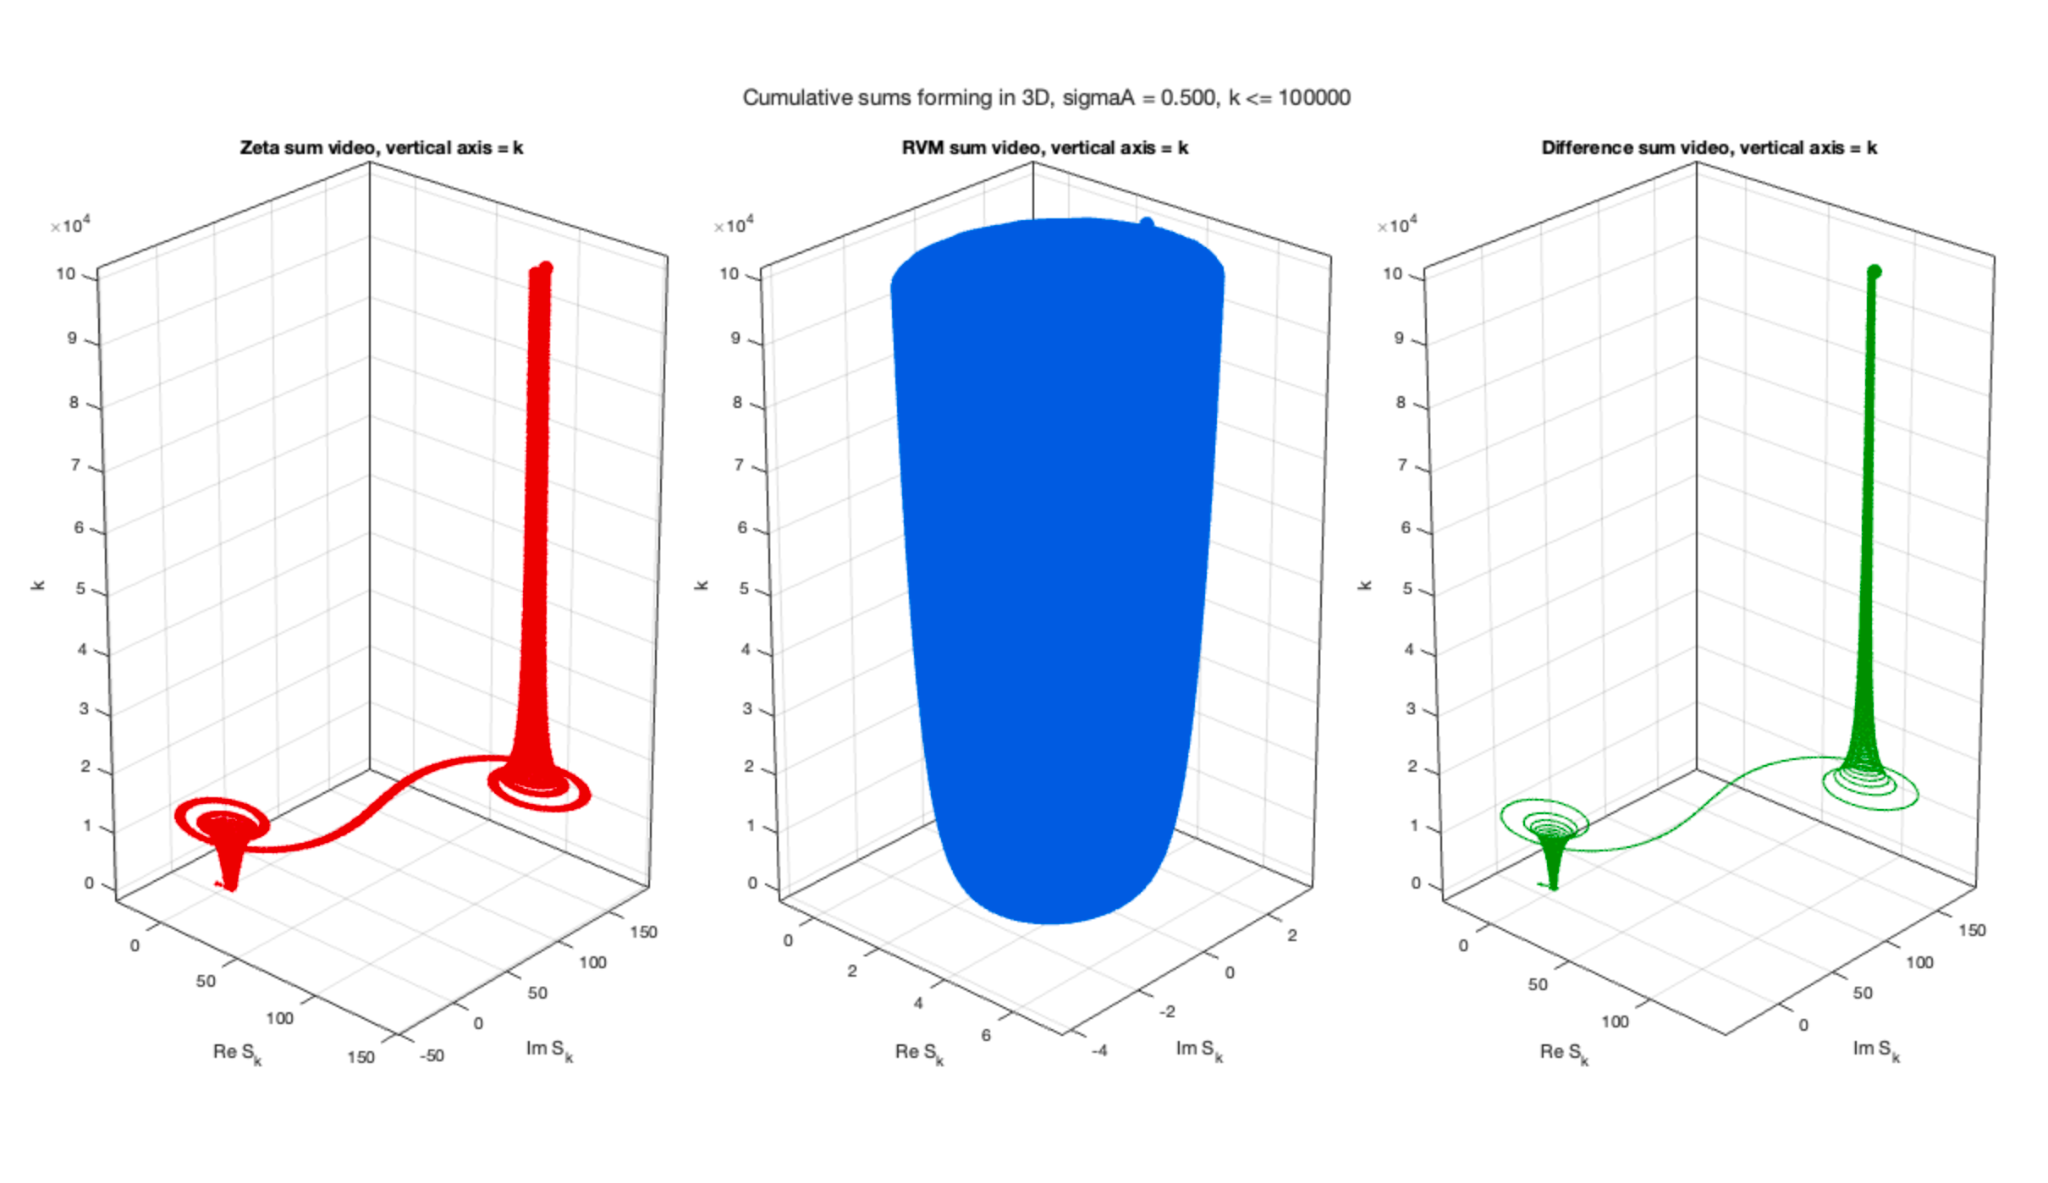
\includegraphics[width=0.95\textwidth]{fig_cumulative_3d.png}
\caption{Ordered cumulative sums for \(k\leq 100000\).  The zeta curve is the primary object; the RVM curve is a smooth control; the difference curve isolates the residual contribution.}
\label{fig:cumulative_3d}
\end{figure}

\begin{figure}[htbp]
\centering
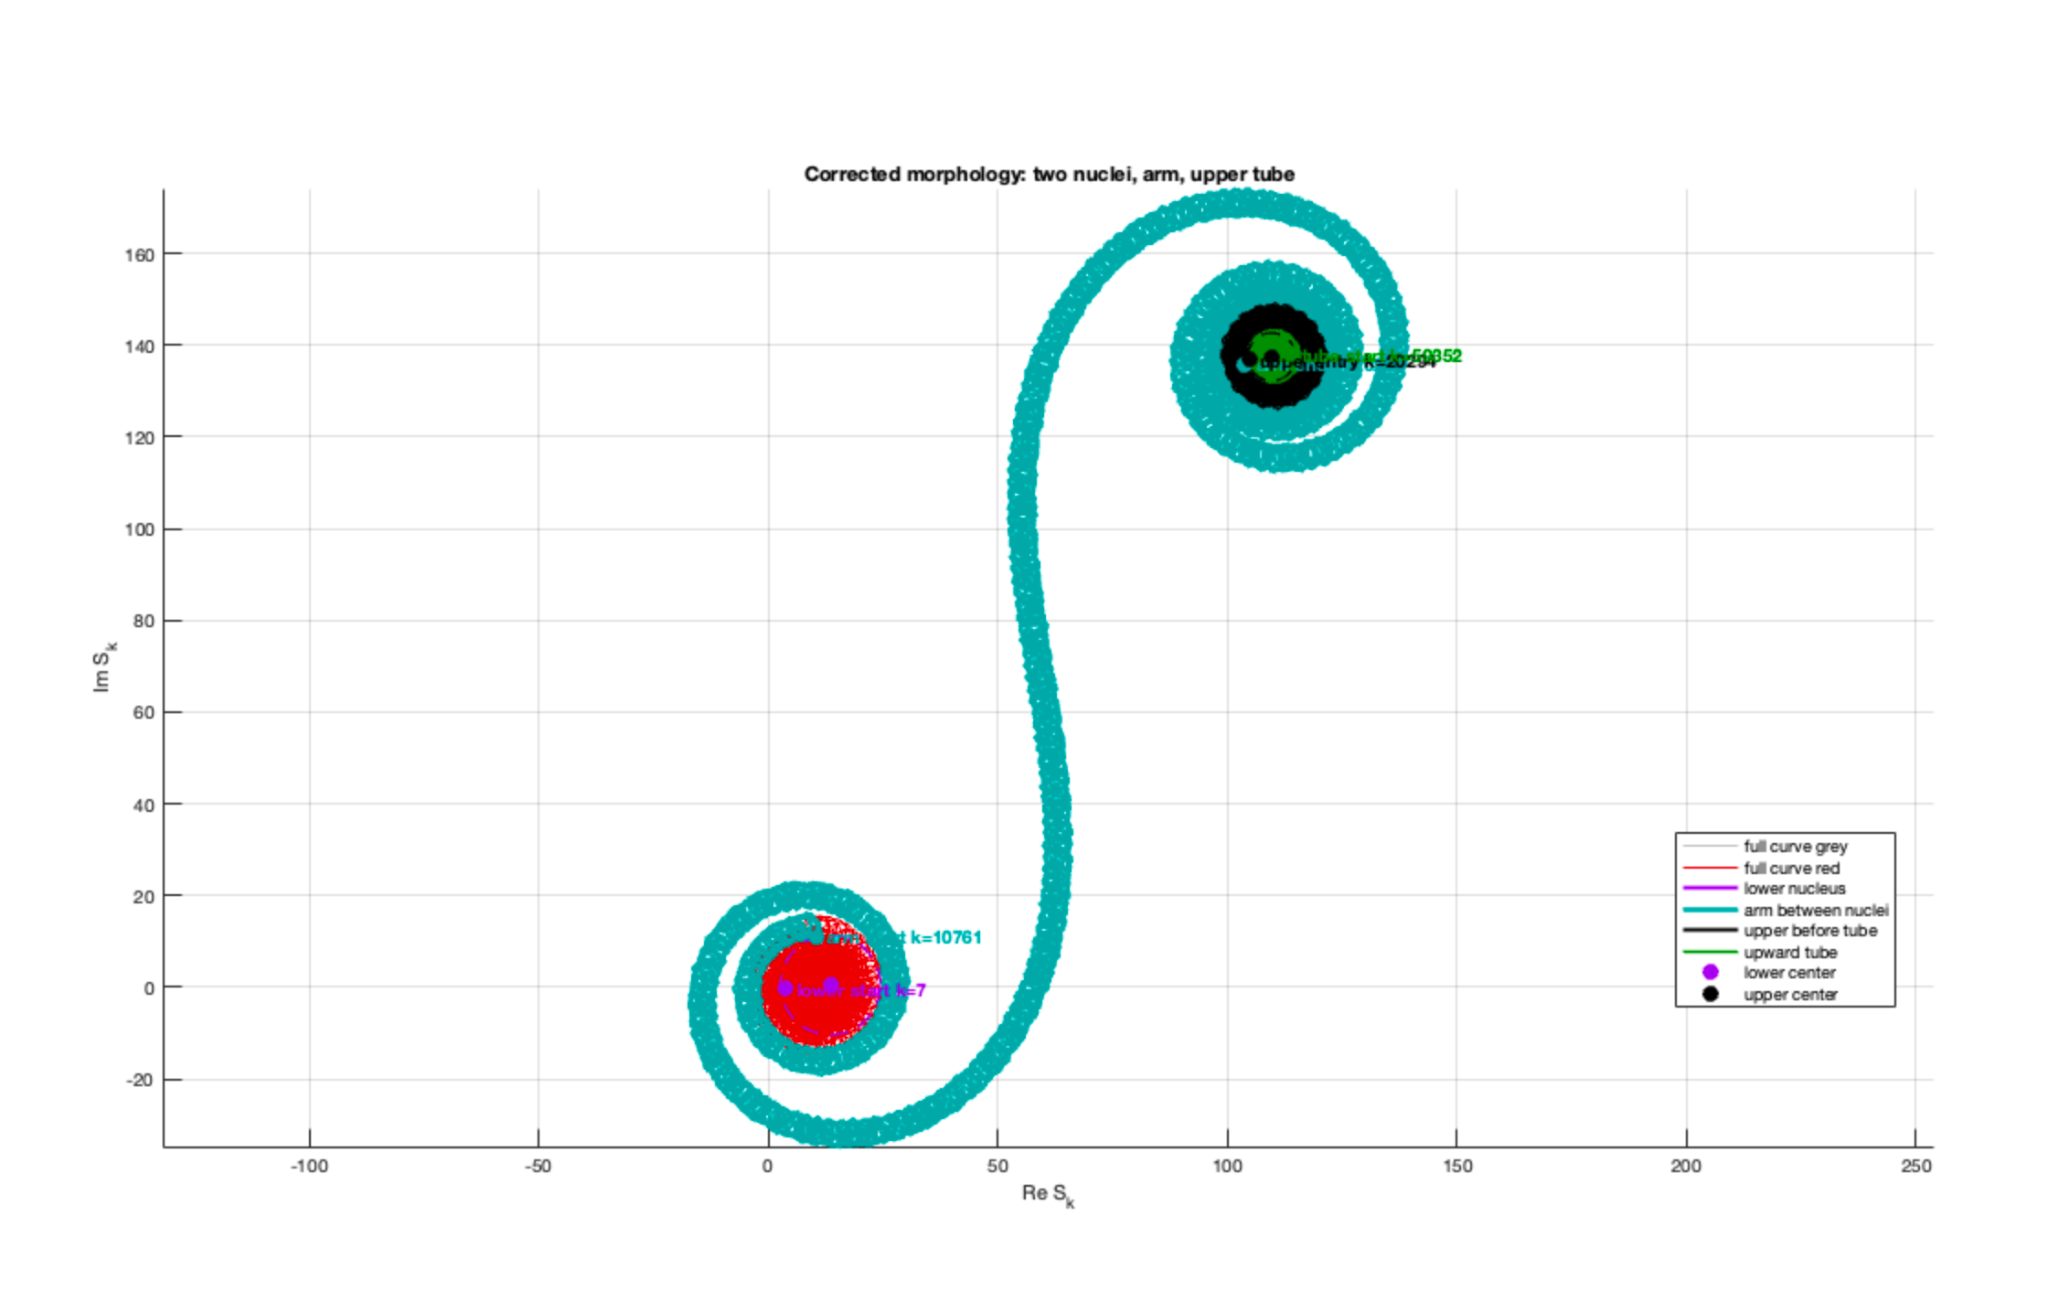
\includegraphics[width=0.95\textwidth]{fig_morphology_2d.png}
\caption{Two-dimensional morphology of the zeta cumulative curve.  The labels are descriptive finite-regime names: lower nucleus, arm, upper entry, and upper tube.}
\label{fig:morphology_2d}
\end{figure}

\begin{definition}
\label{def:descriptive_geometric_regions}
For the finite curve \(S_N^\zeta\), we use the descriptive names lower nucleus, arm, upper entry, and upper tube for the visible regions shown in Figure \ref{fig:morphology_2d}.
\end{definition}


\noindent The names in Definition \ref{def:descriptive_geometric_regions} are finite descriptive labels.  They are not asymptotic theorems.


\begin{experiment}
\label{exp:final_cumulative_values}
For the full data set, \(N=2,001,052\), the computation gives
\begin{align}
S_N^\zeta
&=
107.3092+133.4456i,
\label{eq:exp_final_zeta_value}
\\
S_N^{\RVM}
&=
0.6082-4.0881i,
\label{eq:exp_final_rvm_value}
\\
S_N^{\diff}
&=
106.7010+137.5337i.
\label{eq:exp_final_diff_value}
\end{align}
The corresponding moduli are
\begin{align}
|S_N^\zeta|
&=
171.2396,
\label{eq:exp_final_zeta_modulus}
\\
|S_N^{\RVM}|
&=
4.1331,
\label{eq:exp_final_rvm_modulus}
\\
|S_N^{\diff}|
&=
174.0707.
\label{eq:exp_final_diff_modulus}
\end{align}
The final modulus ratios are
\begin{align}
\frac{|S_N^{\RVM}|}{|S_N^\zeta|}
&=
0.02414,
\label{eq:exp_final_rvm_ratio}
\\
\frac{|S_N^{\diff}|}{|S_N^\zeta|}
&=
1.01653.
\label{eq:exp_final_diff_ratio}
\end{align}
\end{experiment}

\subsection{Ordered window amplitudes}
\label{sec:ordered_window_amplitudes}

\begin{definition}
\label{def:window_amplitude}
For \(x\in\{\zeta,\RVM,\diff\}\), define the window amplitude
\begin{equation}
B_W^x(k)
=
\sum_{j=k}^{k+W-1}z_j^x.
\label{eq:def_window_amplitude}
\end{equation}
For \(x=\diff\), this means
\begin{equation}
B_W^{\diff}(k)
=
\sum_{j=k}^{k+W-1}d_j.
\label{eq:def_residual_window_amplitude}
\end{equation}
\end{definition}

\begin{definition}
\label{def:random_excess}
The random-walk normalized window excess is defined by
\begin{equation}
R_W^x(k)
=
\frac{|B_W^x(k)|}
{\sqrt{W}\,\rms_{j\in[k,k+W-1]}(z_j^x)}.
\label{eq:def_random_excess}
\end{equation}
\end{definition}

\begin{definition}
\label{def:window_cancellation}
The window cancellation statistic is defined by
\begin{equation}
C_W^x(k)
=
1-
\frac{|B_W^x(k)|}{\sum_{j=k}^{k+W-1}|z_j^x|}.
\label{eq:def_window_cancellation}
\end{equation}
\end{definition}


\noindent Values \(R_W^x(k)\) of order one are compatible with a random-walk scale.  Larger values indicate stronger coherent alignment inside the ordered block.  Values \(C_W^x(k)\) close to one indicate strong cancellation, while smaller values indicate stronger internal alignment.


\begin{figure}[htbp]
\centering
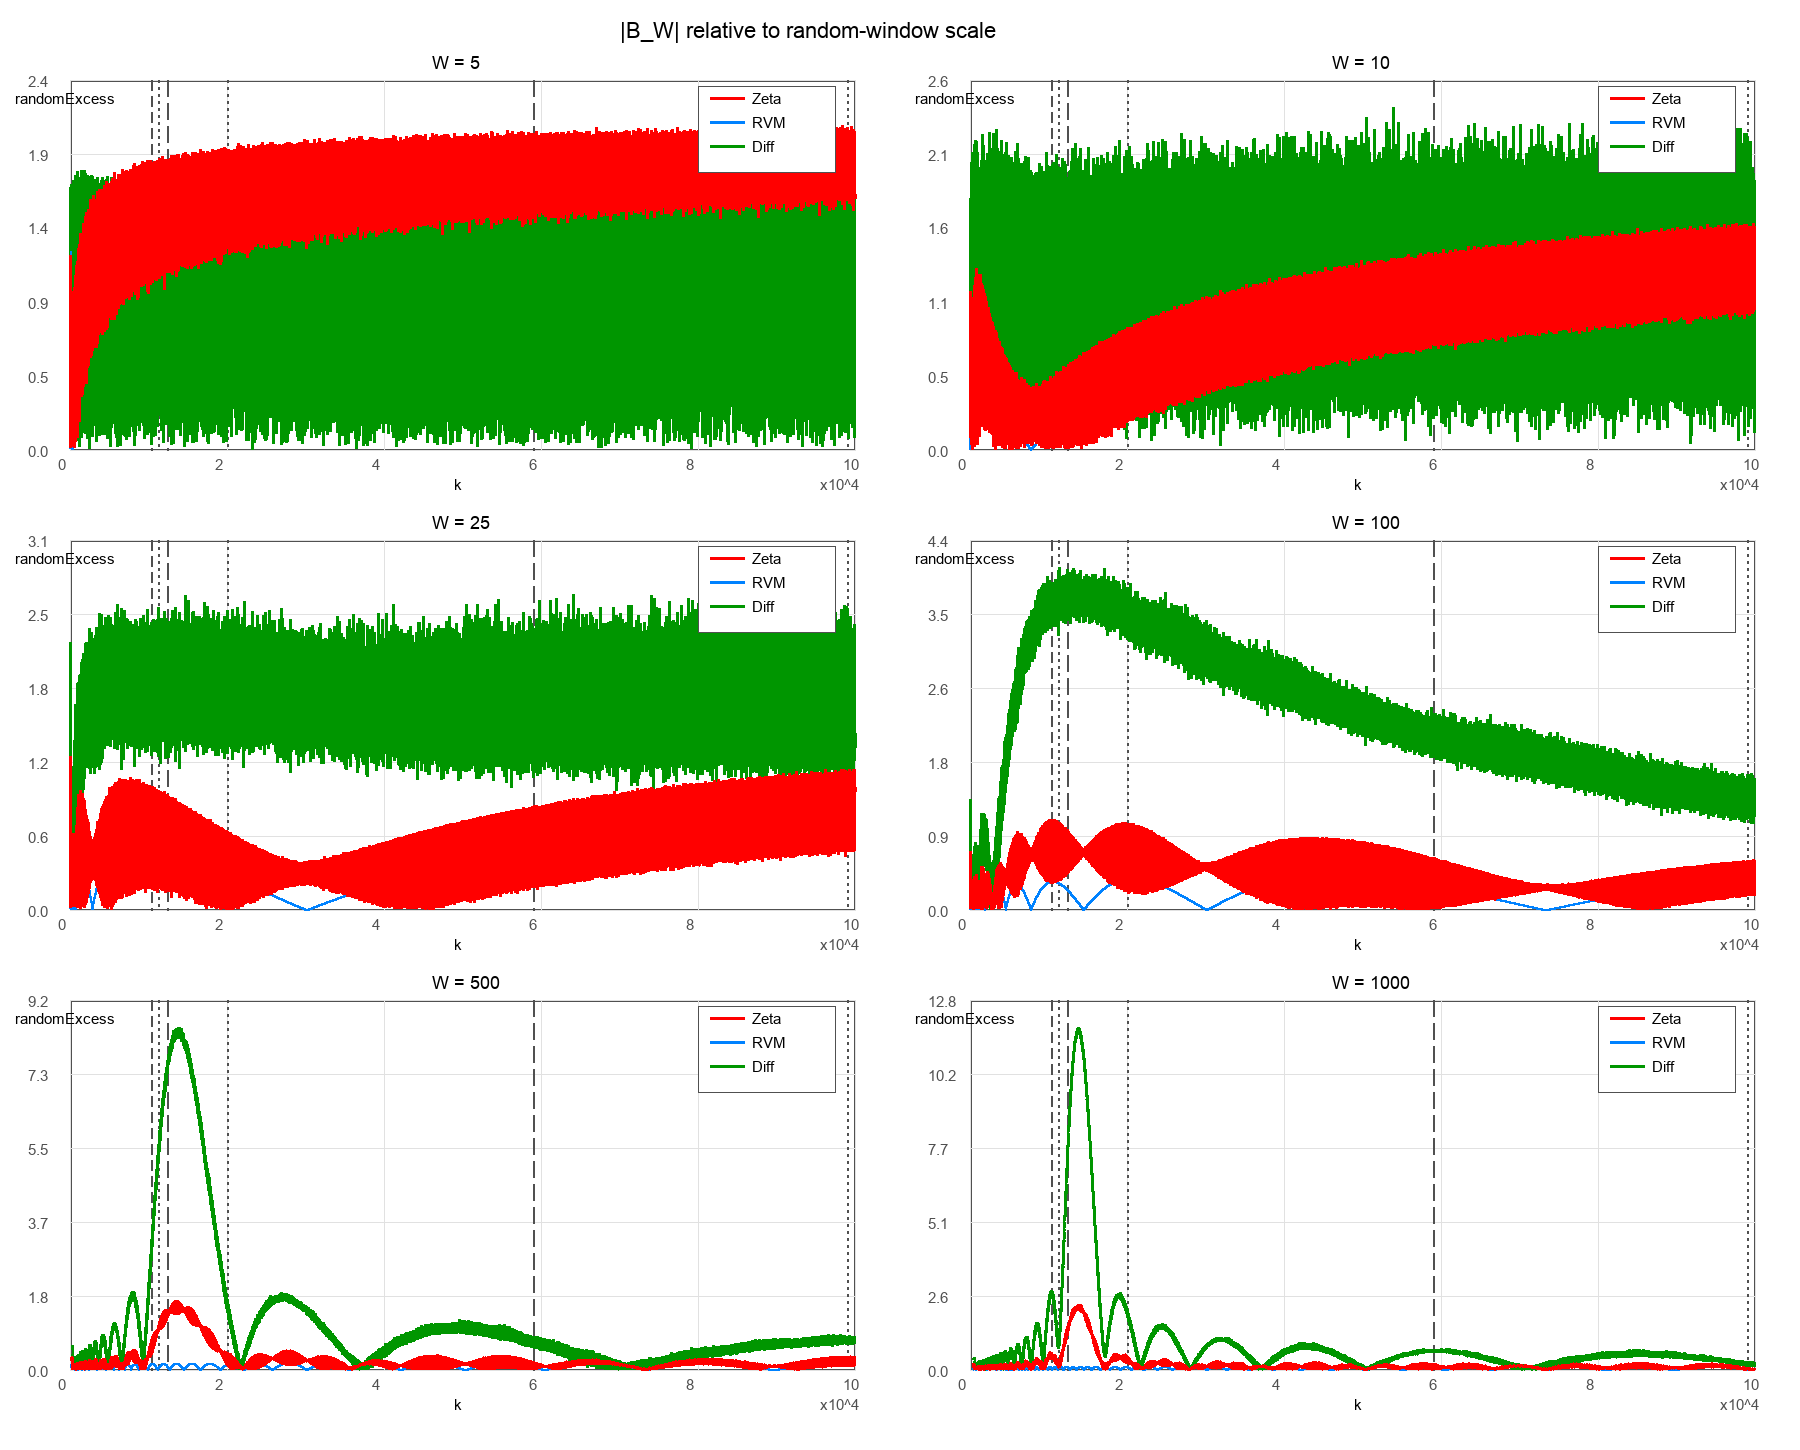
\includegraphics[width=0.98\textwidth]{fig_local_window_diag.png}
\caption{Local window diagnostics for the logarithmic phase-walk transform.  The panels compare zeta, RVM, and residual window behaviour.  The key point is that RVM is not flat: it shows the smooth response imposed by \(\tau_k\), while the zeta and residual signals produce a stronger ordered response beyond the RVM background.}
\label{fig:local_window_diag}
\end{figure}

\begin{figure}[htbp]
\centering
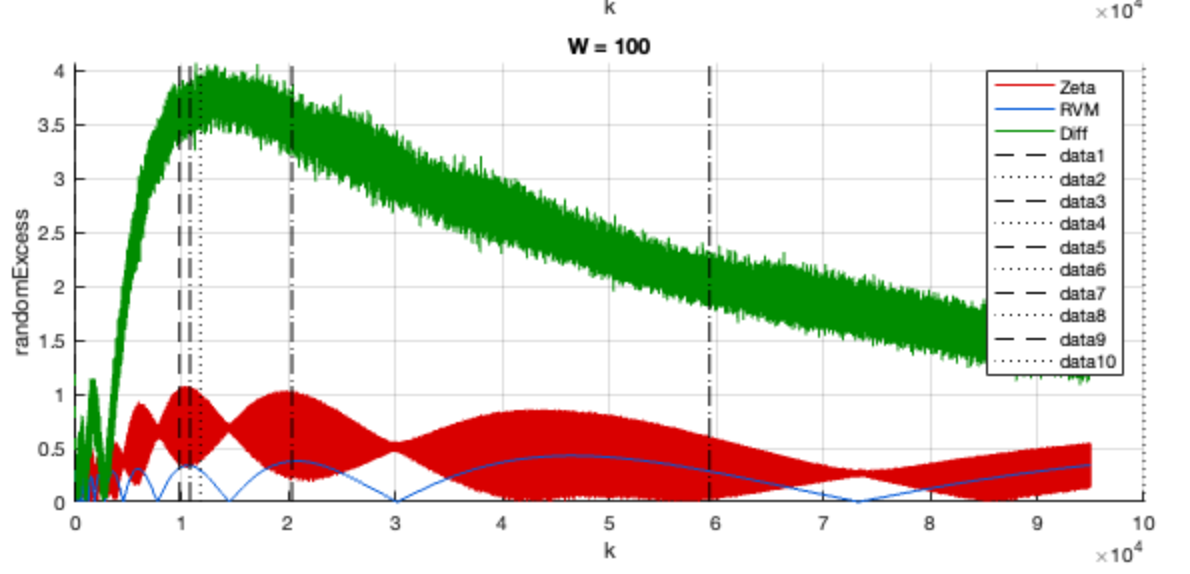
\includegraphics[width=0.95\textwidth]{fig_w100_panel.png}
\caption{The \(W=100\) window panel.  This figure resolves the early finite region where the arm begins to form.  The residual and zeta curves show a stronger ordered response than the RVM control.}
\label{fig:w100_panel}
\end{figure}

\begin{experiment}
\label{exp:residual_window_excess}
For the full data set, \(N=2,001,052\), the residual window excess gives
\begin{align}
\max_k R_{500}^{\diff}(k)
&=
8.4750,
\label{eq:exp_residual_window_500}
\\
\max_k R_{1000}^{\diff}(k)
&=
11.8480,
\label{eq:exp_residual_window_1000}
\\
\max_k R_{2000}^{\diff}(k)
&=
15.8891,
\label{eq:exp_residual_window_2000}
\\
\max_k R_{5000}^{\diff}(k)
&=
11.0871.
\label{eq:exp_residual_window_5000}
\end{align}
The corresponding windows lie in the finite transition region near \(k=1.3\cdot 10^4\) to \(1.5\cdot 10^4\).
\end{experiment}

\begin{experiment}
\label{exp:rvm_window_comparison}
For comparison, the RVM background gives
\begin{align}
\max_k R_{500}^{\RVM}(k)
&=
0.3040,
\label{eq:exp_rvm_window_500}
\\
\max_k R_{1000}^{\RVM}(k)
&=
0.2172,
\label{eq:exp_rvm_window_1000}
\\
\max_k R_{2000}^{\RVM}(k)
&=
0.1561,
\label{eq:exp_rvm_window_2000}
\\
\max_k R_{5000}^{\RVM}(k)
&=
0.09884.
\label{eq:exp_rvm_window_5000}
\end{align}
\end{experiment}

\noindent For any finite sequence \(z_j\), one has
\begin{equation}
|B_W(k)|^2
=
\sum_{a=0}^{W-1}\sum_{b=0}^{W-1}
z_{k+a}\overline{z_{k+b}}.
\label{eq:block_correlation_identity}
\end{equation}
Separating diagonal and off-diagonal terms gives
\begin{align}
|B_W(k)|^2
&=
\sum_{a=0}^{W-1}|z_{k+a}|^2
+
2\operatorname{Re}
\sum_{0\leq a<b\leq W-1}z_{k+a}\overline{z_{k+b}}.
\label{eq:block_correlation_offdiagonal}
\end{align}
The diagonal part sets the random-walk scale.  The off-diagonal part determines whether the ordered block is coherently enhanced or suppressed.  In the present transform, the phase differences are
\begin{equation}
\theta_{k+a}^\zeta-\theta_{k+b}^\zeta
=
\gamma_{k+a}\tau_{k+a}-\gamma_{k+b}\tau_{k+b}.
\label{eq:block_phase_difference}
\end{equation}
Thus the window excess probes ordered phase correlations of the logarithmic phase-walk field.

\subsection{Robustness: Null test with synthetic Selberg-scale noise}
\label{subsec:null_test_synthetic_noise}

\noindent To test whether the observed morphology is reproduced by unstructured perturbations of the correct scale, we use the following null model: inject independent Gaussian noise with the same mean and standard deviation as the measured spectral defect $\delta E_k = \gamma_k - \gamma_k^{\text{RVM}}$ into the smooth RVM sequence, apply the same logarithmic phase-walk transform, and compare both window amplitudes and final cumulative amplitudes.

\begin{definition}
\label{def:synthetic_noise_sequence}
For the RVM ordinates $\gamma_k^{\text{RVM}}$, construct a synthetic perturbed sequence
\begin{equation}
\gamma_k^{\text{noisy}} = \gamma_k^{\text{RVM}} + \varepsilon_k,
\quad
\varepsilon_k \sim \mathcal{N}(\mu_\delta, \sigma_\delta^2),
\label{eq:synthetic_sequence}
\end{equation}
where $\mu_\delta = \mean(\gamma_k - \gamma_k^{\text{RVM}})$ and $\sigma_\delta^2 = \text{var}(\gamma_k - \gamma_k^{\text{RVM}})$ are the empirical mean and variance of the true spectral defect.
\end{definition}

\begin{experiment}
\label{exp:null_test_synthetic_noise}
The independent-noise null was recomputed on the full data set, using all \(2,001,052\) paired Odlyzko and RVM entries.  The plotted paths are downsampled only for display; the numerical values below use the full sequence.  The spectral defect statistics on this full data set are
\begin{align}
\mu_\delta &= -1.6291\times10^{-7}, \label{eq:null_mean_delta} \\
\sigma_\delta &= 0.188066. \label{eq:null_std_delta}
\end{align}

Apply the logarithmic phase-walk transform to three sequences: (i) $\gamma_k$ (true zeta), (ii) $\gamma_k^{\text{RVM}}$ (pure RVM), and (iii) $\gamma_k^{\text{noisy}}$ (RVM + synthetic Gaussian noise of scale $(\mu_\delta, \sigma_\delta)$, seed \(20260631\)).

Compute final cumulative amplitudes and window amplitudes:
\begin{align}
|S_N^\zeta| &= 171.2396, \label{eq:null_zeta_final} \\
|S_N^{\text{RVM}}| &= 4.1331, \label{eq:null_rvm_final} \\
|S_N^{\text{noisy}}| &= 90.8112. \label{eq:null_noisy_final}
\end{align}

For window amplitude $\max_k |B_W^x(k)|$ with $W=500$:
\begin{align}
\text{RVM pure} &: 9.1105, \label{eq:null_window_rvm} \\
\text{RVM + noise} &: 18.4597, \label{eq:null_window_noisy} \\
\text{Zeta real} &: 55.5108. \label{eq:null_window_zeta}
\end{align}
\end{experiment}

\begin{figure}[!t]
\centering
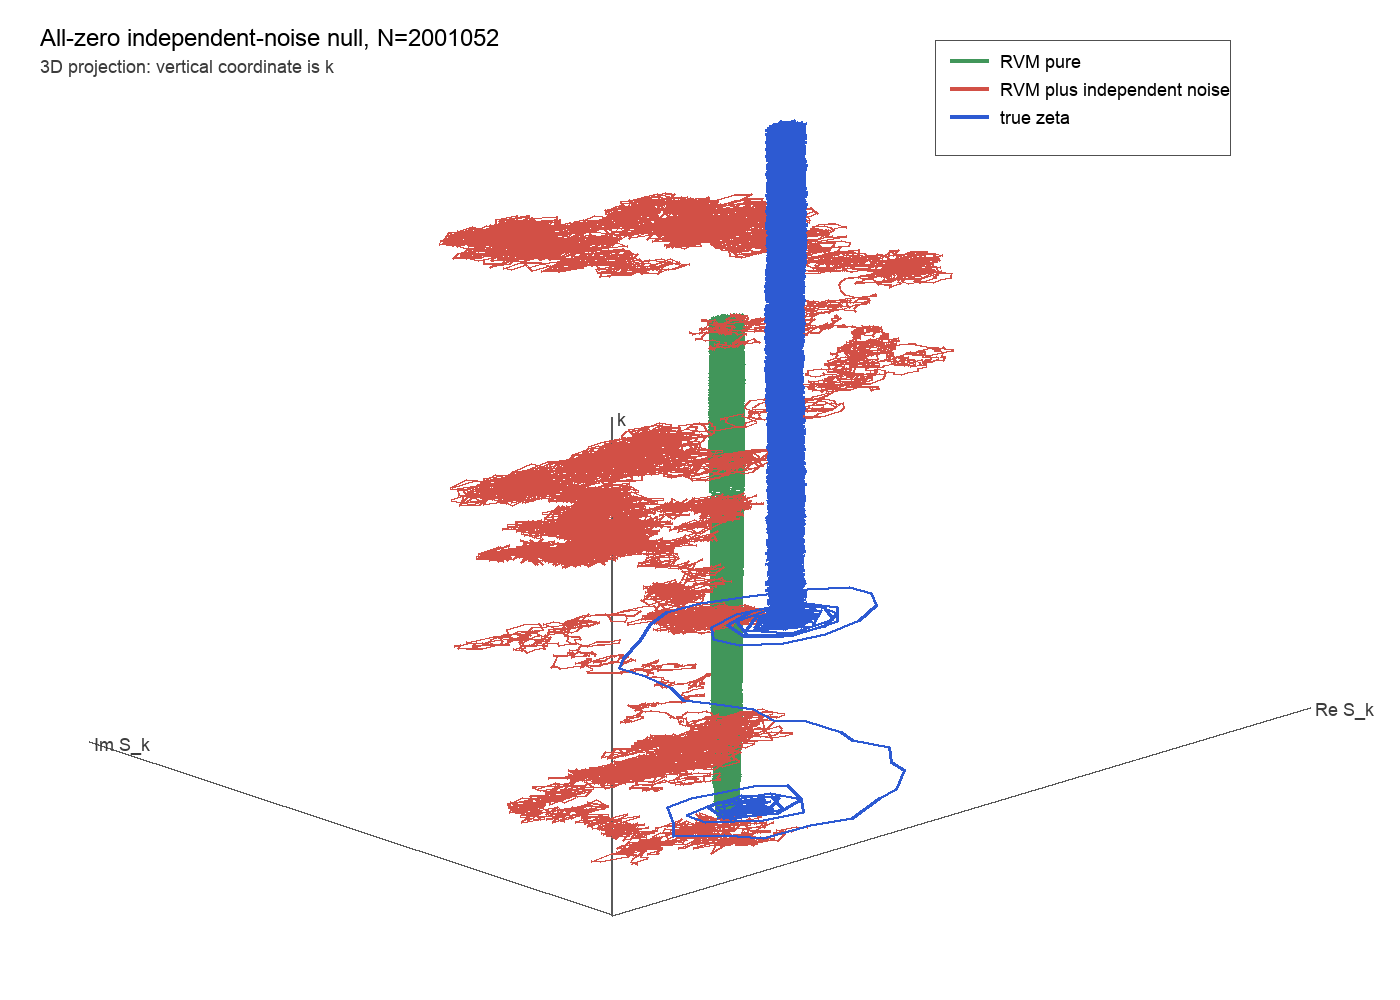
\includegraphics[width=0.95\textwidth]{fig_all_zero_noise_null_paths.png}
\caption{Full-data independent-noise null shown as a 3D cumulative path projection \((\operatorname{Re}S_k,\operatorname{Im}S_k,k)\). The pure RVM background remains confined, the RVM sequence with independent Gaussian perturbations of the empirical zeta--RVM defect scale gives a larger response than pure RVM, and the true zeta sequence gives the strongest ordered window response. For \(W=500\), the maximum window amplitudes are \(9.1105\) for pure RVM, \(18.4597\) for RVM plus independent noise, and \(55.5108\) for the true zeta sequence. The final cumulative moduli are \(4.1331\), \(90.8112\), and \(171.2396\), respectively.}
\label{fig:null_test}
\end{figure}


\noindent The null test should be read in the opposite way from a naive noise explanation.  Independent Gaussian perturbations of the correct one-step scale do not simply reproduce the zeta response.  In the full-data test reported above,
\begin{align}
\max_k |B_{500}^{\RVM}(k)|
&=
9.1105,
\\
\max_k |B_{500}^{\noise}(k)|
&=
18.4597,
\\
\max_k |B_{500}^{\zeta}(k)|
&=
55.5108,
\end{align}
and
\begin{align}
|S_N^{\RVM}|
&=
4.1331,
\\
|S_N^{\noise}|
&=
90.8112,
\\
|S_N^{\zeta}|
&=
171.2396.
\end{align}
Thus the logarithmic transform is sensitive to phase noise of the correct scale, but the zeta sequence is not behaving as independent Gaussian noise.  The true zeta response is much larger than the smooth RVM background and also larger than the independently perturbed RVM sequence in the reported window and final-amplitude diagnostics.  This supports the interpretation that the visible spirals and finite window structures are produced by zeta-specific ordered correlations in the phase defect, not by unstructured noise alone.


\noindent The null model shows two separate effects.  First, fluctuations of the correct scale are sufficient to activate the logarithmic clock.  Second, if those fluctuations are made independent, the response does not match the full zeta morphology.  The true zeta sequence therefore combines Selberg-scale phase fluctuations with ordered correlations that shape the accumulated amplitude.  In this sense the null test separates mere scale sensitivity from the ordered zeta correlations that control the final morphology.

\subsection{Phase portraits and local drift}
\label{sec:phase_portraits_local_drift}

\begin{figure}[H]
\centering
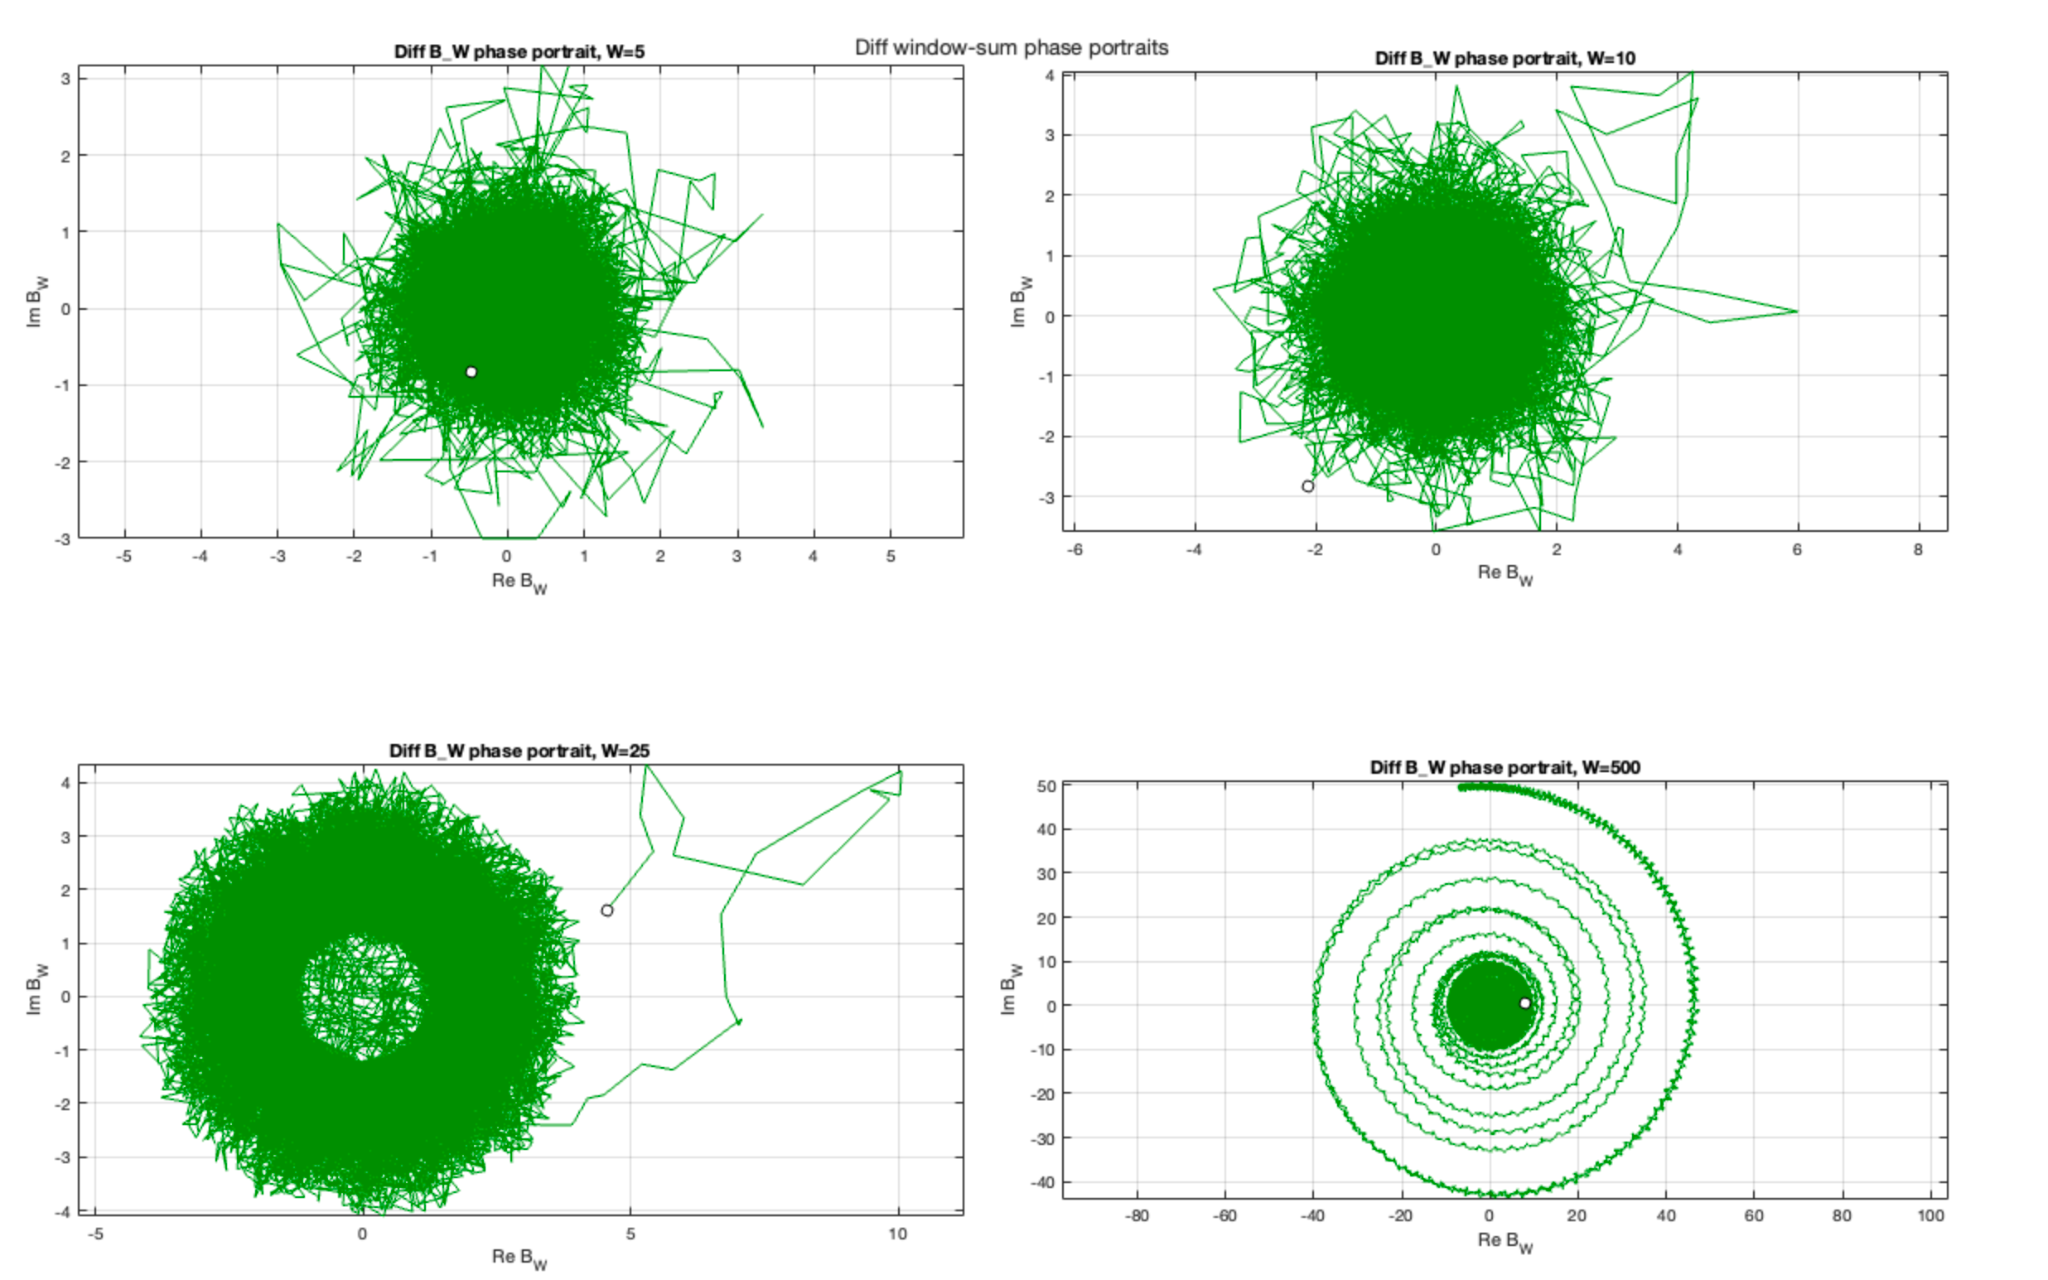
\includegraphics[width=0.88\textwidth]{fig_phase_portraits_diff.png}
\caption{Phase portraits and local drift for selected window sums.  The residual windows form organized loops rather than featureless scatter, and the local drift concentrates near the same finite transition region identified by the window diagnostics.}
\label{fig:phase_portraits_diff}
\end{figure}
\vspace{-0.15cm}


\noindent The phase portraits are not independent assumptions.  They are local projections of the same ordered window amplitudes defined in \eqref{eq:def_window_amplitude}.  Their role is to show that the residual sequence is not featureless after ordered summation.


\subsection{Nearest-neighbor gaps of the transformed function}
\label{sec:nearest_neighbor_gaps}

\begin{definition}
\label{def:direct_vector_gaps}
The direct vector gaps of the transformed zeta and RVM terms are
\begin{align}
D_k^\zeta
&=
|z_{k+1}^\zeta-z_k^\zeta|,
\label{eq:def_zeta_vector_gap}
\\
D_k^{\RVM}
&=
|z_{k+1}^{\RVM}-z_k^{\RVM}|.
\label{eq:def_rvm_vector_gap}
\end{align}
The residual vector gap is
\begin{equation}
D_k^{\diff}
=
|d_{k+1}-d_k|.
\label{eq:def_diff_vector_gap}
\end{equation}
\end{definition}

\begin{definition}
\label{def:functional_angular_gaps}
The angular functional gaps are
\begin{align}
\Delta\theta_k^\zeta
&=
\gamma_{k+1}\tau_{k+1}-\gamma_k\tau_k,
\label{eq:def_zeta_functional_gap}
\\
\Delta\theta_k^{\RVM}
&=
\gamma_{k+1}^{\RVM}\tau_{k+1}-\gamma_k^{\RVM}\tau_k,
\label{eq:def_rvm_functional_gap}
\\
\Delta\theta_k^{\rm resid}
&=
\Delta\theta_k^\zeta-\Delta\theta_k^{\RVM}.
\label{eq:def_resid_functional_gap}
\end{align}
\end{definition}

\begin{definition}
\label{def:locally_unfolded_functional_gap}
For a local unfolding window \(W_{\rm norm}=2000\), define
\begin{align}
s_k^{\rm func,\zeta}
&=
\frac{\Delta\theta_k^\zeta}
{\operatorname{movmedian}(\Delta\theta^\zeta,W_{\rm norm})},
\label{eq:def_sfunc_zeta}
\\
s_k^{\rm func,\RVM}
&=
\frac{\Delta\theta_k^{\RVM}}
{\operatorname{movmedian}(\Delta\theta^{\RVM},W_{\rm norm})}.
\label{eq:def_sfunc_rvm}
\end{align}
\end{definition}

\begin{figure}[!t]
\centering
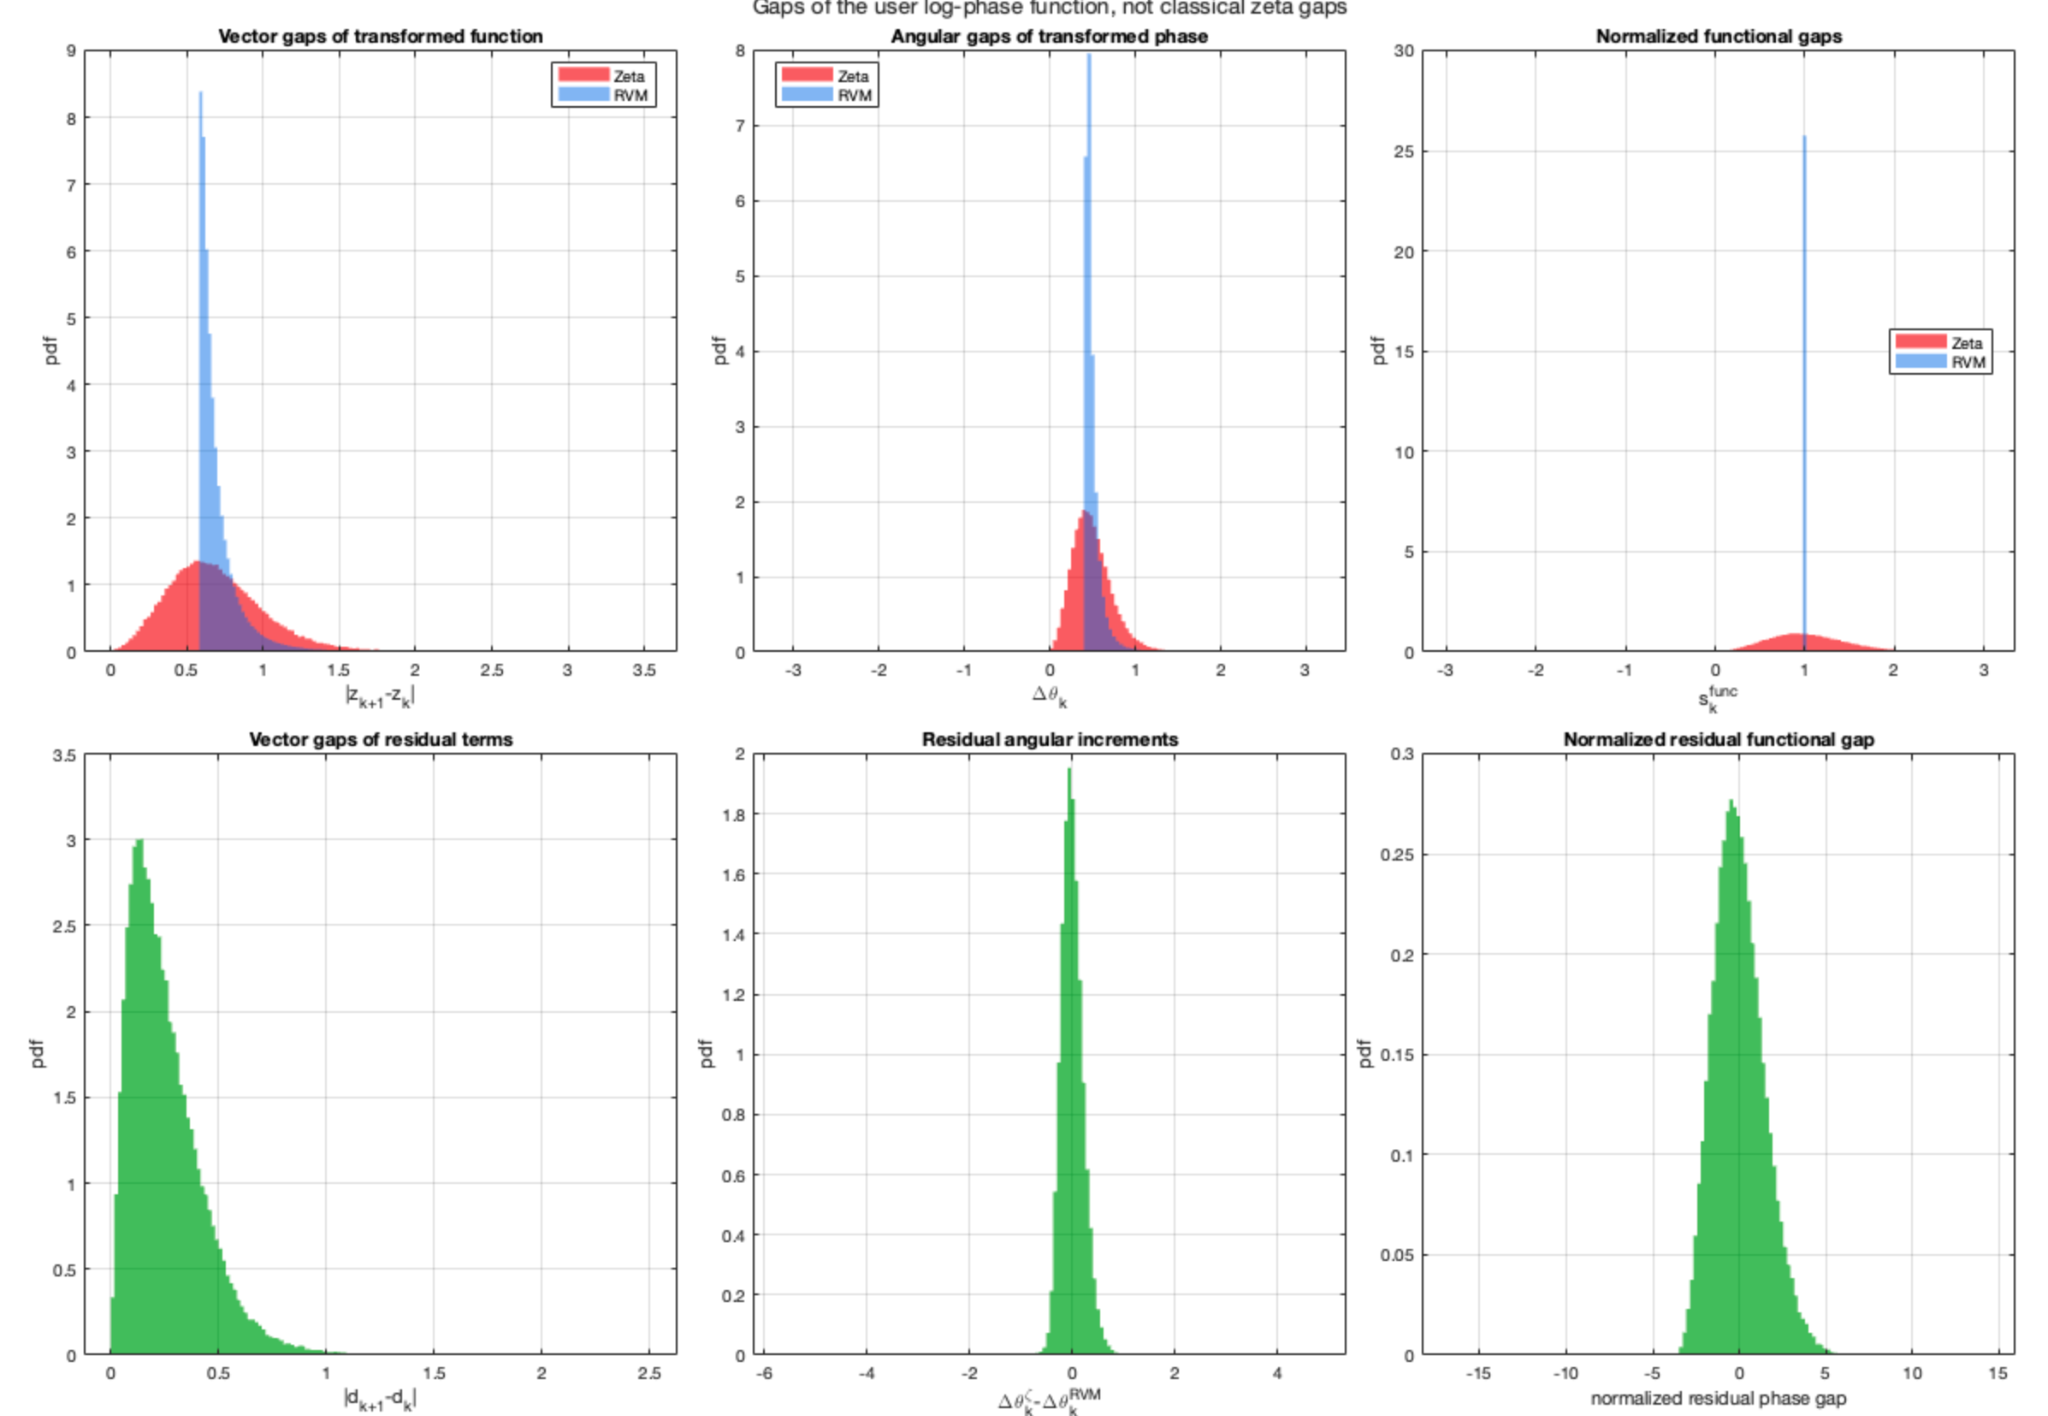
\includegraphics[width=0.92\textwidth]{fig_functional_gaps.png}
\caption{Nearest-neighbor gap diagnostics for the transformed function.  The zeta functional gaps are much broader than the RVM control, while the residual one-step vector gap has its own complex-plane modulus statistics.}
\label{fig:functional_gaps}
\end{figure}

\begin{experiment}
\label{exp:functional_gap_statistics}
For \(N=100000\) and \(W_{\rm norm}=2000\), the direct vector-gap statistics include
\begin{align}
\mean(D^\zeta)
&=
0.6997,
\label{eq:exp_mean_dzeta}
\\
\mean(D^{\RVM})
&=
0.7048,
\label{eq:exp_mean_drvm}
\\
\mean(D^{\diff})
&=
0.2569.
\label{eq:exp_mean_ddiff}
\end{align}
The standard deviations are
\begin{align}
\operatorname{std}(D^\zeta)
&=
0.3374,
\label{eq:exp_std_dzeta}
\\
\operatorname{std}(D^{\RVM})
&=
0.1720,
\label{eq:exp_std_drvm}
\\
\operatorname{std}(D^{\diff})
&=
0.1754.
\label{eq:exp_std_ddiff}
\end{align}
For the locally normalized functional angular gaps,
\begin{align}
\operatorname{std}(s^{\rm func,\zeta})
&=
0.4470,
\label{eq:exp_std_sfunc_zeta}
\\
\operatorname{std}(s^{\rm func,\RVM})
&=
0.04462.
\label{eq:exp_std_sfunc_rvm}
\end{align}
Thus the zeta functional gaps have approximately ten times the standard deviation of the RVM control after local normalization.
\end{experiment}

\subsection{Rayleigh local residual gaps}
\label{sec:rayleigh_local_residual_gaps}

\begin{definition}
\label{def:mean_normalized_diff_gap}
The mean-normalized residual vector gap is
\begin{equation}
s_k^{\rm diffvec}
=
\frac{|d_{k+1}-d_k|}{\mean_j |d_{j+1}-d_j|}.
\label{eq:def_mean_normalized_diff_gap}
\end{equation}
\end{definition}

\begin{definition}
\label{def:comparison_laws}
The comparison laws used in the nearest-neighbor residual test are
\begin{align}
p_{\GUE}(s)
&=
\frac{32}{\pi^2}s^2e^{-4s^2/\pi},
\label{eq:def_gue_wigner_surmise}
\\
p_{\Poisson}(s)
&=
e^{-s},
\label{eq:def_poisson_law}
\\
p_{\Rayleigh}(s)
&=
\frac{s}{\sigma_R^2}
\exp\left(-\frac{s^2}{2\sigma_R^2}\right),
\qquad
\sigma_R=\sqrt{\frac{2}{\pi}}.
\label{eq:def_rayleigh_law}
\end{align}
\end{definition}

\begin{figure}[H]
\centering
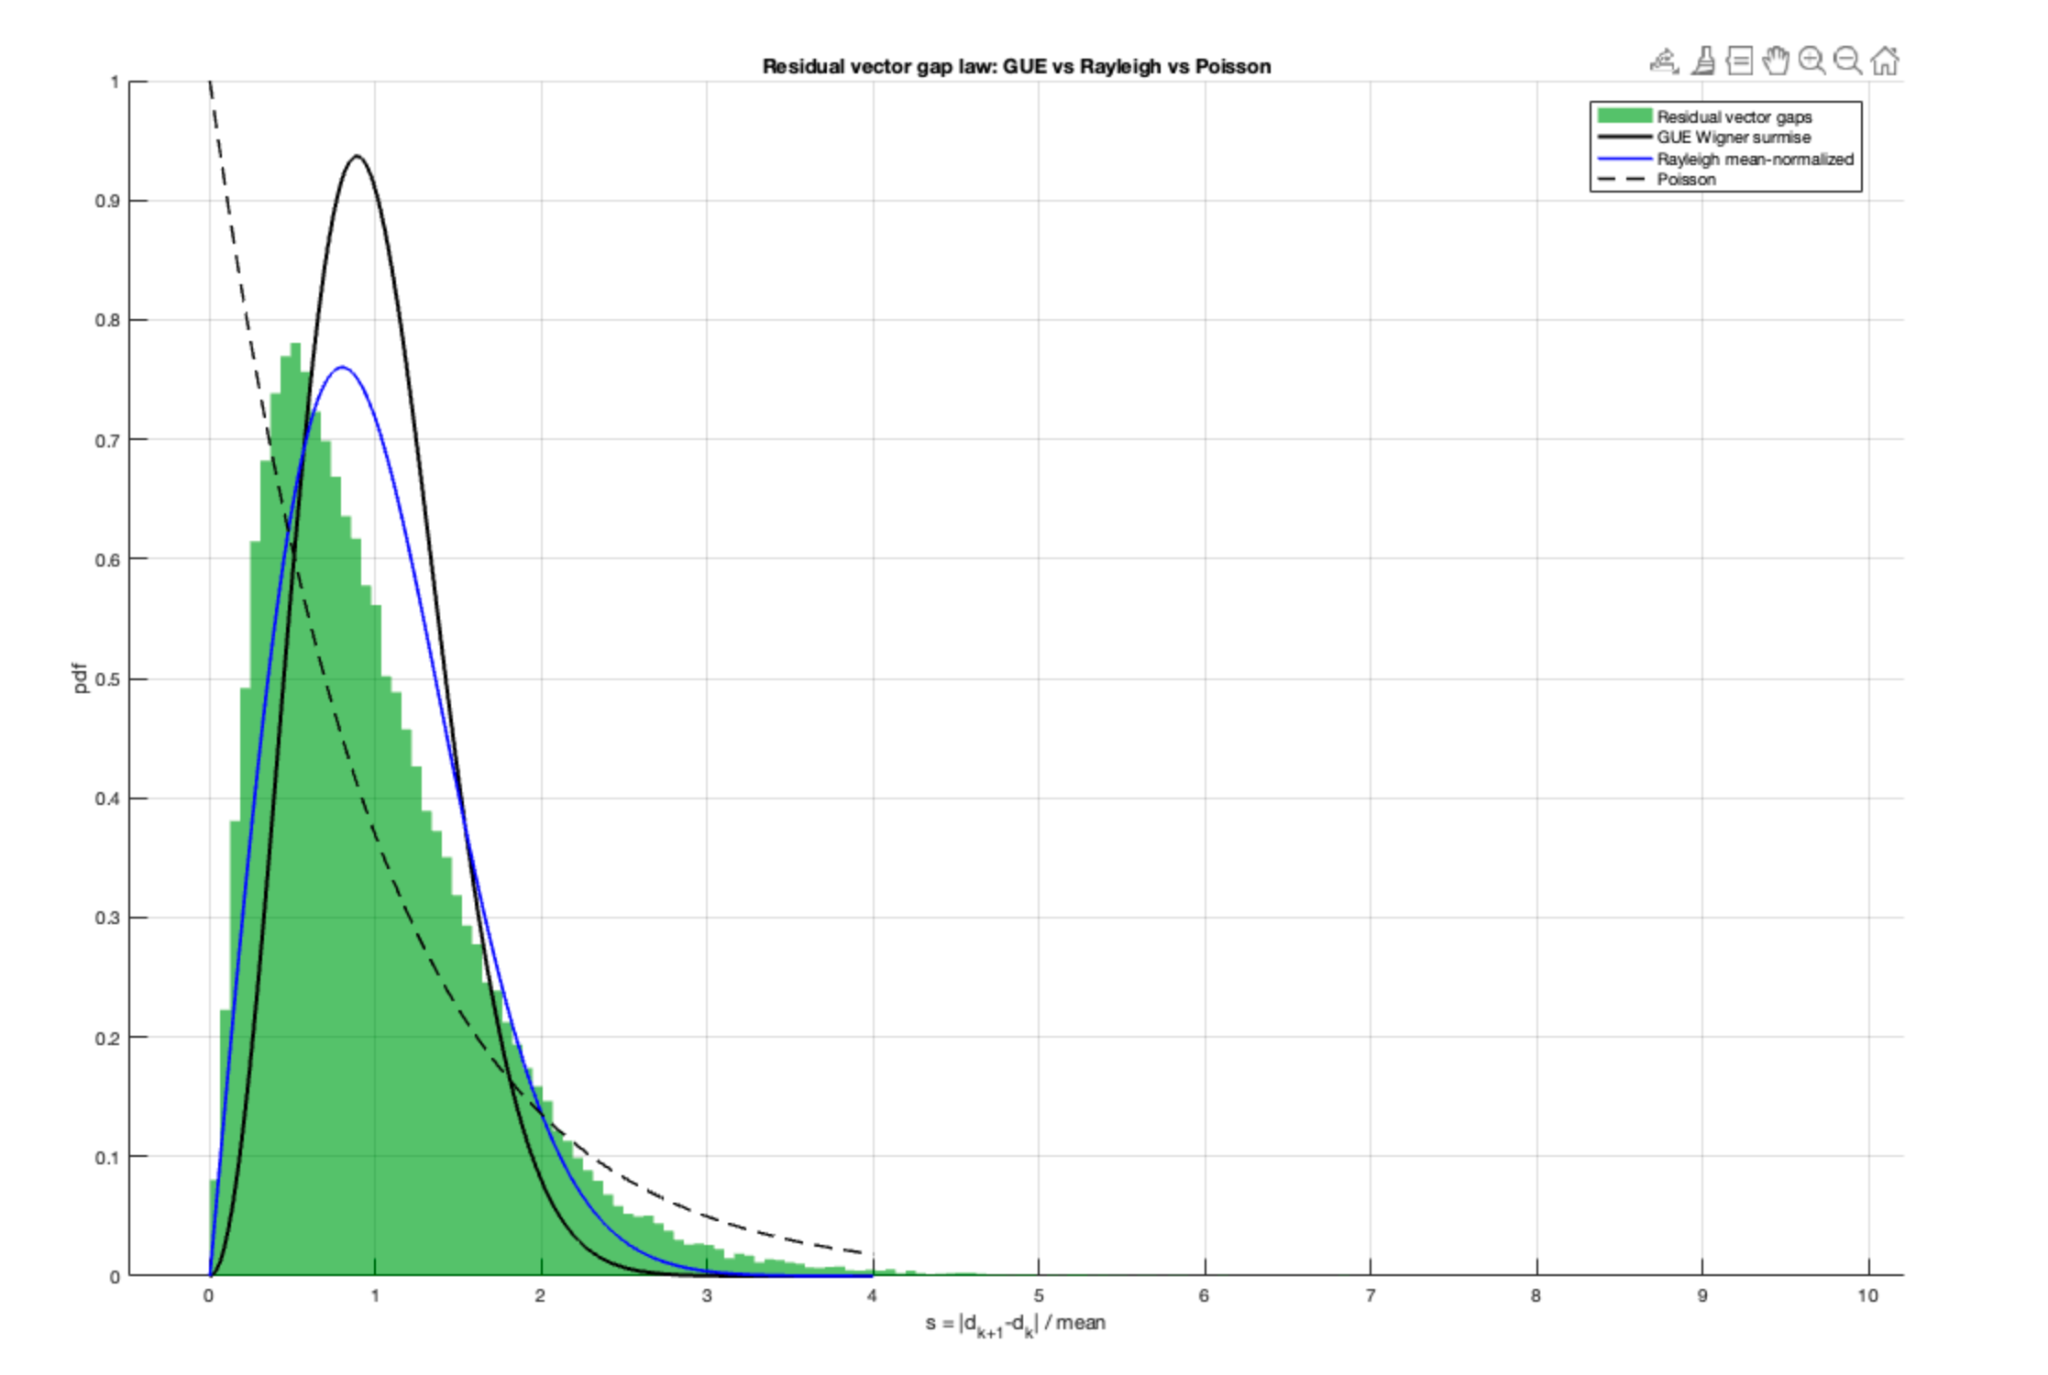
\includegraphics[width=0.84\textwidth]{fig_rayleigh_gap_law.png}
\caption{Nearest-neighbor residual vector gaps of the transformed function.  After normalization by their mean, the residual gaps \(|d_{k+1}-d_k|\) are compared with the GUE Wigner surmise, Poisson spacing, and the mean-normalized Rayleigh planar-modulus benchmark.}
\label{fig:rayleigh_gap_law}
\end{figure}
\vspace{-0.15cm}

\begin{experiment}
\label{exp:rayleigh_gap_law}
For \(N=100000\), the mean raw residual vector gap is
\begin{equation}
\mean_k |d_{k+1}-d_k|
=
0.2569,
\label{eq:exp_mean_raw_diff_gap}
\end{equation}
and the median normalized residual vector gap is
\begin{equation}
\median(s^{\rm diffvec})
=
0.8493.
\label{eq:exp_median_normalized_diff_gap}
\end{equation}
The Kolmogorov--Smirnov distances are
\begin{align}
\KS_{\GUE}
&=
0.2752,
\label{eq:exp_ks_gue}
\\
\KS_{\Rayleigh}
&=
0.08390,
\label{eq:exp_ks_rayleigh}
\\
\KS_{\Poisson}
&=
0.1555.
\label{eq:exp_ks_poisson}
\end{align}
The near-zero CDF exponent, fitted from
\begin{equation}
P(s\leq \varepsilon)
\sim
\varepsilon^\alpha,
\label{eq:exp_near_zero_cdf_law}
\end{equation}
is
\begin{equation}
\alpha
=
1.963.
\label{eq:exp_near_zero_cdf_exponent}
\end{equation}
\end{experiment}


\noindent The value \eqref{eq:exp_near_zero_cdf_exponent} is close to the Rayleigh CDF exponent \(2\), not to the GUE nearest-neighbor exponent \(3\), and not to the Poisson exponent \(1\).  The residual difference \(d_{k+1}-d_k\) is a complex planar quantity; the Re/Im component audit reported below shows isotropic component geometry for these transformed residual increments, so the modulus is compared with the Rayleigh planar benchmark.

\subsection{Odlyzko-style GUE control versus residual laws}
\label{sec:odlyzko_style_gue_control}

The preceding Rayleigh comparison concerns the transformed residual sequence, not the original zero spacings.  To verify that this distinction is not an artefact of normalization, an Odlyzko-style control test was run on three objects:
\begin{enumerate}[label=(\roman*)]
\item the unfolded zero ordinates \(X_k=N_0(\gamma_k)\), with \(N_0\) as in \eqref{eq:introduction_mean_rvm_count},
\item the raw scalar defect \(\delta_k=\gamma_k-r_k\),
\item the exact transformed residual
\[
d_k=
\exp(\tau_k/2+i r_k\tau_k)
\left(\exp(i\tau_k\delta_k)-1\right).
\]
\end{enumerate}
The same paper clock
\[
\tau_k=\pi\frac{\log\log k}{\log k}
\]
was used for the transformed object.  The zero ordinates were tested both by nearest-neighbor spacings and by local unfolded pairs \(0<X_j-X_i\leq L_{\max}\), with \(L_{\max}=3,5,10\) and bin width \(0.05\).  The residual objects were tested by the corresponding index-local pair distances after normalization by their nearest-neighbor mean.

\begin{experiment}
\label{exp:odlyzko_style_control}
The run used \(N=2,001,052\).  The unfolded zeros give the expected GUE--Montgomery control.  The nearest-neighbor zero spacings have KS distance \(0.01252\) to the GUE Wigner surmise, compared with \(0.09959\) to Rayleigh and \(0.29197\) to the exponential law.  For local unfolded zero pairs, the Montgomery-pair KS distances were \(0.00565\), \(0.00317\), and \(0.00151\) for \(L_{\max}=3,5,10\), respectively.

The raw and transformed residual objects behave differently.  For nearest-neighbor residual distances, the raw defect is closest to the exponential comparison in this test (KS \(0.08780\)), while the transformed residual gives KS distances \(0.16966\) to GUE, \(0.13627\) to Rayleigh, and \(0.13156\) to the exponential law.  For index-local transformed residual pairs, however, Rayleigh is clearly the closest of the three simple comparison laws:
\begin{center}
\begin{tabular}{c|ccc}
\toprule
\(L_{\max}\) & Montgomery/GUE KS & Rayleigh KS & Exponential KS \\
\midrule
3  & 0.34384 & 0.06822 & 0.16728 \\
5  & 0.53960 & 0.05635 & 0.17810 \\
10 & 0.74158 & 0.06818 & 0.16914 \\
\bottomrule
\end{tabular}
\end{center}
If Erlang-2 is added as a fourth one-dimensional control, its KS distances for the transformed local-pair radii are \(0.03802\), \(0.04952\), and \(0.04209\) for \(L_{\max}=3,5,10\), respectively.
\end{experiment}

\paragraph{Erlang-2 radial control.}
\label{par:erlang2_radial_control}
A further Re/Im component audit supports the planar interpretation.  For the exact transformed residual, the local-pair increment cloud is circular to the precision of the audit: at \(L_{\max}=3\), the correlation between real and imaginary parts is \(1.996\times10^{-4}\), the covariance eigenvalue ratio is \(1.0011\), and the circularity coefficient is \(5.689\times10^{-4}\).  The same isotropic component geometry holds for \(L_{\max}=5\) and \(L_{\max}=10\).  Thus Rayleigh is the natural planar comparison for a complex residual modulus, which is the statistic emphasized in this article.  The auxiliary centered radial variable \(|Z-\overline Z|\) is a stricter one-dimensional summary: in that audit Erlang-2 gives a smaller KS distance than Rayleigh for the aggregated local-pair radii.  For \(L_{\max}=3\), the centered-radial KS distances are \(0.09242\) for Rayleigh and \(0.02420\) for Erlang-2; for \(L_{\max}=5\), they are \(0.05851\) and \(0.04875\); and for \(L_{\max}=10\), they are \(0.06846\) and \(0.04202\).  Erlang-2 is therefore retained as a one-dimensional radial control, while the main geometric interpretation remains planar: the log-phase residual has isotropic complex increment geometry and Rayleigh is the appropriate benchmark for the residual modulus.


\subsection{Scale-clock parametrization}
\label{sec:optional_scale_clock_interpretation}

\noindent Introduce the scale coordinate
\begin{equation}
u=
\log k,
\label{eq:scale_coordinate_u}
\end{equation}
Then the logarithmic proper time becomes
\begin{equation}
\tau_k
=
\pi\frac{\log u}{u}.
\label{eq:proper_time_scale_coordinate}
\end{equation}
This displays \(\tau_k\) as a scale-dependent phase clock in the coordinate \(u\).  The point is only that different spectral levels are advanced with different effective phase speeds under the transform.


\noindent This parametrization is not an additional assumption.  It only rewrites the clock already present in the definition of the observable.  The numerical claims of the article are the definitions of the transform, the comparison with the RVM control, and the finite window and gap diagnostics.


\subsection{Finite computational observation and all-zero null tests}
\label{sec:finite_computational_observation}

\begin{experiment}
\label{exp:finite_residual_window_excess_summary}
For the full data set, \(N=2,001,052\), the residual window excess values in Experiment \ref{exp:residual_window_excess} imply the finite observations
\begin{align}
\max_k R_{500}^{\diff}(k)
&=
8.4750,
\label{eq:obs_residual_excess_500_exact}
\\
\max_k R_{1000}^{\diff}(k)
&=
11.8480,
\label{eq:obs_residual_excess_1000_exact}
\\
\max_k R_{2000}^{\diff}(k)
&=
15.8891.
\label{eq:obs_residual_excess_2000_exact}
\end{align}
These are finite output values, not a theorem about all heights.
\end{experiment}

\begin{experiment}
\label{exp:all_zero_sign_amplitude_coordinate_audit}
An all-zero audit was carried out on all \(2,001,052\) paired entries of the zero and RVM binary files, using the active index range \(k=3,\ldots,2,001,052\) and no shifted clock.  Thus
\[
\tau_k=\pi\frac{\log\log k}{\log k}
\]
was used exactly as in the definition of the observable.  Write
\[
\delta_k=\gamma_k-r_k,\qquad
s_k=\operatorname{sgn}(\delta_k),\qquad
A_k=|\delta_k|,
\]
and
\[
W_k=i\tau_k\exp(\tau_k/2+i r_k\tau_k).
\]
The linearized residual is \(d_k^{\rm lin}=A_ks_kW_k\), while the exact residual is
\[
d_k^{\rm exact}
=
\exp(\tau_k/2+i r_k\tau_k)
\left(\exp(i\tau_k\delta_k)-1\right).
\]
For the exact residual cumulative sum, the final modulus was \(174.0707\), the maximum cumulative modulus was \(204.8496\), the mean normalized amplitude was \(1.1833\), and the median normalized amplitude was \(1.0113\).  For the linearized residual the corresponding values were \(163.3911\), \(194.2243\), \(1.1094\), and \(0.9448\).  The endpoint discrepancy between exact and linear cumulative residuals was \(11.9599\), giving a relative endpoint error \(0.0687\).  The real and imaginary one-step correlations between the exact and linear terms were \(0.9947\) and \(0.9947\), respectively.
\end{experiment}

\noindent The raw signed defect already has very strong scalar cancellation before the logarithmic phase coordinate is applied.  In the same all-zero audit,
\[
\left|\sum_{k=3}^{N}\delta_k\right|
=
0.3260,
\qquad
\mean Q(\delta)
=
0.00197,
\]
whereas the pure sign sum has final absolute value \(630\) and mean \(Q=0.3310\).  Thus the sign \(s_k\) and the scalar cancellation in \(\delta_k=A_ks_k\) are properties of the zeta--RVM defect itself.  The logarithmic phase coordinate does not create this sign structure; it projects the already signed scalar defect into a complex residual geometry.

\begin{experiment}
\label{exp:all_zero_null_ablation}
Several null transformations were then applied to separate sign, amplitude, phase coordinate, and order effects.  In pointwise random-sign nulls, \(s_k\) was replaced by independent \(\pm1\) signs while \(A_k\) and \(W_k\) were kept fixed.  The raw signed scalar walk \(A_ks_k\) was far below these random-sign nulls in mean \(Q\) (real \(0.00197\), null mean \(0.7059\) in the local audit), confirming that the scalar defect is not an arbitrary independent-sign sequence.  By contrast, the projected exact residual had mean \(Q=1.1833\) against a point-sign null mean \(0.8855\) in the same audit.  Block sign flips with block sizes from \(500\) to \(200000\) did not give an extreme mean-\(Q\) separation in this run; the observed mean \(Q\) lay within the sampled block-null ranges.  Circular sign shifts gave projected-linear mean \(Q=1.1094\) against null mean \(1.3094\), while amplitude shuffling gave null mean \(0.8725\).  These tests indicate that the scalar cancellation is already present in \(\delta_k\), while the complex geometry depends on the joint alignment of signed defect, amplitude, and phase coordinate rather than on any one factor alone.
\end{experiment}

\begin{experiment}
\label{exp:all_zero_order_and_window_tests}
Order tests further show that the natural ordering is part of the morphology.  The exact residual in natural order has mean \(Q=1.1833\).  A global permutation of terms gives mean \(Q=0.7632\), reversing the order gives mean \(Q=0.0146\), circular shifting gives mean \(Q=0.6495\), sorting by amplitude gives mean \(Q=0.7795\), and sorting by phase gives mean \(Q=26.4278\).  Thus the final endpoint is invariant under permutation, but the path geometry and normalized accumulation are not.  The strongest all-zero window excesses for the exact residual were
\[
\max R_{500}=8.4750,\qquad
\max R_{1000}=11.8480,\qquad
\max R_{2000}=15.8891,
\]
with the maxima located in the early transition region \(k\approx 1.3\times10^4\).  The all-zero local residual-gap comparison gave KS distances \(0.1015\) for the mean-normalized Rayleigh law, \(0.1697\) for the GUE Wigner surmise, and \(0.1315\) for the exponential law, so Rayleigh remained the best of these three simple comparisons on the full data set.
\end{experiment}

\noindent The computation up to \(N=2,001,052\) shows a stabilized upper-tube regime after the early transitions.  Larger-height computations would be needed to determine whether further phase-block reorganizations produce new arms, tubes, or relocations of the cumulative geometry.


\subsection{Auxiliary real-coordinate response profile}
\label{sec:counting_coordinate_response_profiles}

The logarithmic phase-walk observable studied in the preceding sections uses the ordinate coordinate \(\gamma_k\).  This section records a separate construction involving the real coordinate \(\sigma\).  Its role is different from the phase-walk observable: it is a signed real-coordinate response built around the critical coordinate \(1/2\).  It is defined without assuming RH.  If an actual zero is supplied with real part \(\sigma_k\neq1/2\), the associated signed weight records that displacement from the critical line.  If RH holds, the supplied real-coordinate displacement is zero for every nontrivial zero and the signed weight vanishes term by term in the natural limiting sense.


\noindent The parameter \(\beta\) in \(D_X(\beta)\) is a supplied real coordinate.  Therefore a plot of \(D_X(\beta)\) as \(\beta\) varies should be read as a response profile of the construct, not as a statement that zeros exist at those externally chosen real parts.  This is the correct scope of the object.  The construct excludes, by definition, any off-critical contribution unless an off-critical real coordinate is supplied.  Its potential value is as a formal starting point for analytic refinements involving the real coordinate, not as a standalone numerical search procedure.


\subsection{Completed zeta function and local normalization}
\label{subsec:completed_zeta_local_normalization}

\begin{definition}
\label{def:completed_zeta_xi}
The completed zeta function is
\begin{equation}
\xi(s)
=
\frac{1}{2}s(s-1)\pi^{-s/2}\Gamma\left(\frac{s}{2}\right)\zeta(s),
\label{eq:completed_zeta_xi}
\end{equation}
and satisfies the functional equation
\begin{equation}
\xi(s)=\xi(1-s).
\label{eq:completed_zeta_functional_equation}
\end{equation}
\end{definition}


\noindent For real \(\sigma\) and \(\gamma\), the functional equation and the reality of \(\xi\) on the real axis give
\begin{equation}
|\xi(\sigma+i\gamma)|
=
|\xi(1-\sigma+i\gamma)|.
\end{equation}
This is a standard symmetry of the completed zeta function, not a detector by itself.


\begin{definition}
\label{def:general_nontrivial_zero}
Write a nontrivial zero as
\begin{equation}
\rho_k
=
\sigma_k+i\gamma_k,
\label{eq:general_nontrivial_zero}
\end{equation}
ordered by nondecreasing positive ordinate and counted with multiplicity.  Its real displacement from the critical line is
\begin{equation}
\Delta\sigma_k
=
\sigma_k-\frac{1}{2}.
\label{eq:zero_real_displacement_from_critical_line}
\end{equation}
\end{definition}

\begin{definition}
\label{def:Ck_delta_coefficient}
Let \(m_k\) be the multiplicity of the zero \(\rho_k\) of \(\xi\), and let
\begin{equation}
a_k
=
\frac{\xi^{(m_k)}(\rho_k)}{m_k!}.
\label{eq:leading_taylor_coefficient_xi}
\end{equation}
Thus \(a_k\neq0\), and locally
\begin{equation}
\xi(s)
=
a_k(s-\rho_k)^{m_k}
+
O\left((s-\rho_k)^{m_k+1}\right).
\label{eq:xi_local_multiplicity_expansion}
\end{equation}
For a supplied real displacement \(\delta\neq0\), define the multiplicity-normalized coefficient
\begin{equation}
C_k(\delta)
=
\left|
\frac{\xi(\rho_k+\delta)}{a_k\delta^{m_k}}
\right|^{-2},
\label{eq:Ck_delta_coefficient}
\end{equation}
whenever the expression is finite and nonzero.  This coefficient is positive by construction whenever it is defined.  In the simple-zero case \(m_k=1\), \(a_k=\xi'(\rho_k)\), so \eqref{eq:Ck_delta_coefficient} reduces to the usual first-derivative normalization.
\end{definition}

\subsection{Counting coordinate and response profile}
\label{subsec:counting_coordinate_response_profile}

\begin{definition}
\label{def:zero_counting_function}
Let
\begin{equation}
N(T)
=
\#\{k:0<\gamma_k\leq T\}
\label{eq:zero_counting_function}
\end{equation}
be the zero-counting function, with zeros counted according to the ordering convention above.  At the ordinate \(\gamma_k\), the finite counting coordinate is
\begin{equation}
u_k
=
\log N(\gamma_k)
=
\log k.
\label{eq:logarithmic_counting_coordinate_Dx}
\end{equation}
\end{definition}

\begin{definition}
\label{def:DX_beta_balance}
For \(X>0\) and a supplied real coordinate \(\beta\), set
\begin{equation}
\Delta\sigma
=
\beta-\frac{1}{2}
\label{eq:real_displacement_from_critical_line}
\end{equation}
and define the response profile
\begin{equation}
D_X(\beta)
=
\sum_{\gamma_k\leq X}
C_k(\Delta\sigma)
\left(
N(\gamma_k)^{2\Delta\sigma}
-
N(\gamma_k)^{-2\Delta\sigma}
\right).
\label{eq:DX_beta_balance}
\end{equation}
Equivalently, using \(N(\gamma_k)=k\),
\begin{equation}
D_X(\beta)
=
\sum_{k\leq N(X)}
C_k(\Delta\sigma)
\left(
k^{2\Delta\sigma}-k^{-2\Delta\sigma}
\right).
\label{eq:DX_beta_indexed_balance}
\end{equation}
\end{definition}


\noindent Since \(u_k=\log k\), each signed weight difference is
\begin{equation}
k^{2\Delta\sigma}-k^{-2\Delta\sigma}
=
2\sinh(2\Delta\sigma u_k).
\end{equation}
Consequently, for fixed externally supplied \(\Delta\sigma\), the sign of each defined nonzero summand is the sign of \(\Delta\sigma\).  This sign property is algebraic and contains no information about whether a zero actually has real part \(\beta\).


\noindent If \(\beta\) is chosen externally, for example \(\beta=0.9\), the sign of the summands is dictated by the supplied displacement \(\beta-1/2\).  Such a calculation describes the response of the formal real-coordinate profile at that supplied coordinate.  It is different from evaluating the construct on an actual zero with known real part \(\sigma_k\).  The distinction is essential: an externally supplied \(\beta\) probes the profile; an actual \(\sigma_k\) records the real-coordinate displacement of a supplied zero.


\subsection{Critical involution and the role of the actual real parts}
\label{subsec:critical_involution_actual_real_parts}


\noindent Under the critical involution \(s\mapsto1-s\), the real displacement changes sign,
\begin{equation}
\Delta\sigma
\longmapsto
-\Delta\sigma,
\end{equation}
while the counting coordinate remains the positive coordinate
\begin{equation}
u_k=\log k>0.
\end{equation}
Thus the involution exchanges
\begin{equation}
e^{2\Delta\sigma u_k}
\longleftrightarrow
 e^{-2\Delta\sigma u_k}
\label{eq:critical_involution_weight_exchange_corrected}
\end{equation}
by changing \(\Delta\sigma\), not by replacing the actual coordinate \(u_k\) with \(-u_k\).


\noindent It is not correct to identify the actual counting coordinate with a transformation \(u_k\mapsto -u_k\).  The equality \(u_k=-u_k\) would force \(u_k=0\), which is not the case for \(k>1\).  The only valid exchange is the weight exchange in \eqref{eq:critical_involution_weight_exchange_corrected} at fixed positive \(u_k\).


\begin{definition}
\label{def:actual_real_coordinate_response}
If a zero \(\rho_k=\sigma_k+i\gamma_k\) is supplied with its actual real coordinate, define its actual real displacement by \eqref{eq:zero_real_displacement_from_critical_line}.  The associated per-zero signed response is defined by
\begin{equation}
\mathcal{D}_k
=
0
\qquad
\text{if }\Delta\sigma_k=0,
\label{eq:actual_per_zero_response_critical}
\end{equation}
and by
\begin{equation}
\mathcal{D}_k
=
C_k(\Delta\sigma_k)
\left(k^{2\Delta\sigma_k}-k^{-2\Delta\sigma_k}\right)
\qquad
\text{if }\Delta\sigma_k\neq0,
\label{eq:actual_per_zero_response_offcritical}
\end{equation}
whenever the coefficient is defined.  This quantity uses the actual \(\sigma_k\), not an externally chosen \(\beta\).
\end{definition}


\noindent If RH holds, then \(\Delta\sigma_k=0\) for every nontrivial zero and \(\mathcal{D}_k=0\) term by term by \eqref{eq:actual_per_zero_response_critical}.  If a zero is supplied with \(\sigma_k\neq1/2\), then \(\Delta\sigma_k\neq0\) and \eqref{eq:actual_per_zero_response_offcritical} gives a signed response whose sign records the side of the critical line on which that supplied zero lies.  Thus the construct is built without assuming RH, and it responds immediately to an off-critical real coordinate if such a zero is supplied.


\noindent The article therefore contains two complementary coordinates.  The logarithmic phase-walk observable uses \(\gamma_k\) and reveals ordered phase geometry in the ordinate direction.  The real-coordinate response profile uses \(\sigma_k\) as a supplied coordinate and records displacement from the critical line.  Its relevance is that it gives a clean starting point for refinements in which the real-coordinate response is connected to deeper analytic structure of \(\xi\).


\subsection{The tau-gauge lateral zero detector}
\label{subsec:tau_lateral_zero_detector}

\noindent The phase clock used in the phase-walk is not intrinsically tied to the restriction \(\sigma_k=1/2\).  For a finite indexed set of supplied zeros
\[
\rho_k=\beta_k+i\gamma_k,
\]
define the lateral displacement and tau-gauge vertical coordinate by
\begin{equation}
x_k=\beta_k-\frac{1}{2},
\qquad
u_k^{\tau}=\gamma_k\tau_k.
\label{eq:tau_lateral_coordinates}
\end{equation}
In the main observable, \(\tau_k\) appears in the phase factor \(e^{i\gamma_k\tau_k}\).  In the following detector, the same quantity \(u_k^{\tau}\) is used as the vertical coordinate of a regularized lateral field.  This is a lateral zero detector in the following literal sense: once a finite multiset of zeros is supplied, the field sources and the positive moments below are supported exactly on those zero coordinates; the moments then distinguish purely critical-line data from data containing at least one off-critical zero.

\noindent For \(\varepsilon>0\), set
\begin{equation}
K_{\varepsilon}^{\tau}(x,u;x',u')
=
\frac{x-x'}
{(x-x')^2+(u-u')^2+\varepsilon^2}.
\label{eq:tau_lateral_kernel}
\end{equation}
This is the regularized \(x\)-derivative of the planar potential after the vertical pullback \(u=\gamma\tau(\gamma)\).  It is a Euclidean kernel in the declared \((x,u)\) gauge, not in the original \((x,\gamma)\) coordinate.  Thus the nonlinear tau gauge changes the metric interpretation, while preserving a well-defined regularized field in \((x,u)\).

\noindent A critical-line zero gives a wall source \(x'=0\):
\begin{equation}
K_{\varepsilon}^{\tau}(x,u;0,v)
=
\frac{x}{x^2+(u-v)^2+\varepsilon^2},
\label{eq:critical_wall_source}
\end{equation}
which is odd in \(x\) and even in \(u-v\):
\begin{equation}
K_{\varepsilon}^{\tau}(-x,u;0,v)=-K_{\varepsilon}^{\tau}(x,u;0,v),
\qquad
K_{\varepsilon}^{\tau}(x,2v-u;0,v)=K_{\varepsilon}^{\tau}(x,u;0,v).
\label{eq:critical_wall_source_symmetry}
\end{equation}
A symmetric off-line pair at lateral displacement \(\pm a\) and vertical coordinate \(v\) gives the lateral mode
\begin{equation}
M_{a,\varepsilon}^{\tau}(x,u;v)
=
\frac{x-a}{(x-a)^2+(u-v)^2+\varepsilon^2}
+
\frac{x+a}{(x+a)^2+(u-v)^2+\varepsilon^2}.
\label{eq:off_line_lateral_mode}
\end{equation}
This mode has the same critical-axis symmetries,
\begin{equation}
M_{a,\varepsilon}^{\tau}(-x,u;v)=-M_{a,\varepsilon}^{\tau}(x,u;v),
\qquad
M_{a,\varepsilon}^{\tau}(x,2v-u;v)=M_{a,\varepsilon}^{\tau}(x,u;v),
\label{eq:off_line_lateral_mode_symmetry}
\end{equation}
with the sign symmetry imposed by the involution \(x\mapsto -x\) around the critical line.  The mode is a lateral source class rather than a wall source on the critical axis, so the tau gauge separates critical-line sources from off-line lateral sources.

\noindent A positive lateral moment on a finite window \(W\) is
\begin{equation}
\mathcal L_{\alpha}^{\tau}(W)
=
\sum_{\rho_k\in W}
m_k x_k^2
\exp\left[-\alpha\left(x_k^2+(u_k^{\tau})^2\right)\right],
\qquad \alpha>0,
\label{eq:positive_tau_lateral_moment}
\end{equation}
where \(m_k\) is the multiplicity.  Every summand in \eqref{eq:positive_tau_lateral_moment} is nonnegative, and the exponential factor is strictly positive.  Therefore
\begin{equation}
\mathcal L_{\alpha}^{\tau}(W)\geq0,
\qquad
\mathcal L_{\alpha}^{\tau}(W)=0
\Longleftrightarrow
x_k=0
\quad\text{for every included zero}.
\label{eq:positive_tau_lateral_moment_zero_criterion}
\end{equation}
Equivalently, the moment is strictly positive as soon as the window contains at least one supplied zero with \(\beta_k\neq1/2\).

\noindent A symmetric displaced version is
\begin{equation}
\mathcal G_{\alpha,h}^{\tau}(W)
=
2\sum_{\rho_k\in W}
m_k
\exp\left[-\alpha\left(x_k^2+(u_k^{\tau})^2\right)\right]
\left(\cosh(2\alpha h x_k)-1\right),
\qquad \alpha>0,\ h\neq0.
\label{eq:gemini_tau_lateral_moment}
\end{equation}
Since \(\cosh t-1\geq0\), this also satisfies
\begin{equation}
\mathcal G_{\alpha,h}^{\tau}(W)\geq0,
\qquad
\mathcal G_{\alpha,h}^{\tau}(W)=0
\Longleftrightarrow
x_k=0
\quad\text{for every included zero}.
\label{eq:gemini_tau_lateral_moment_zero_criterion}
\end{equation}
Thus the tau-gauge lateral zero detector is compatible with the RH-restricted computations, where \(x_k=0\), but it is formally defined for supplied zeros with arbitrary real part.  It gives a second diagnostic use of the same clock: phase accumulation in the main walk, and tau-gauge placement of supplied zero coordinates inside a lateral potential-field detector.


\section{Conclusions}
\label{sec:conclusion}

We have defined and analyzed a logarithmic phase-walk observable for zeta-zero ordinates, compared it with the RVM background, and demonstrated its structural properties on the first 2,001,052 Odlyzko zero ordinates.  The null tests were computed on the same full paired data set and separate the smooth RVM control, independently perturbed RVM data, and the ordered zeta response.

\textbf{Main findings:} In the all-zero audit, the one-step residual vector gaps are closer to the Rayleigh comparison (KS$_{\text{Rayleigh}}=0.1015$) than to the GUE Wigner-surmise comparison (KS$_{\text{GUE}}=0.1697$) or the exponential comparison (KS$_{\text{Exp}}=0.1315$). This Rayleigh behaviour is observed in a different object from the usual Montgomery--Odlyzko statistic: GUE describes spacings of zero ordinates, while Rayleigh is used here as the planar modulus benchmark for isotropic complex residual increments after the logarithmic phase-walk transform. This is the first reported detection of such planar Rayleigh behaviour for this transformed zeta--RVM residual observable. The coherent signal emerges at the level of ordered window amplitudes, with residual window excess reaching factors of 8--16 above the random-walk scale for $W=500$--$2000$.

\textbf{Limitations.} The main limitation of the present paper is that the proposed observable is exploratory and its conclusions are supported by a finite computational range rather than by an asymptotic theorem.  Within the computed region, however, the transformed zeta zeros and the transformed RVM background display clearly distinct behaviour.  This distinction opens a new perspective on zeta-zero structure and on which yet-unobserved properties of the zeta sequence, beyond its smooth RVM approximation, may be responsible for the effect.

\textbf{Scope and generality.} The construction is not limited to zeta. Any ordered quantum chaotic spectrum, random-matrix spectrum, or spectral model with a smooth background and a level-dependent clock can be analyzed by the same method.  Possible applications include quantum chaos and disordered systems, where GUE-type local statistics are already used but ordered phase accumulation may contain additional information. The observable reveals phase-interference structure that local spacing statistics discard because they ignore ordering. The persistence of the observed planar Rayleigh and window-excess behaviour for the full infinite zero sequence remains open.

\textbf{Two-coordinate response.} Section \ref{sec:counting_coordinate_response_profiles} adds a complementary real-coordinate construct using the abscissa $\sigma_k$. It is defined independently of RH: on the critical line its signed response vanishes, while a supplied zero with $\sigma_k\neq1/2$ gives a nonzero signed response. Section \ref{subsec:tau_lateral_zero_detector} introduces the corresponding tau-gauge lateral zero detector. The same \(\tau\)-kernel used in the phase-walk can therefore be applied to supplied zero data with arbitrary real parts, giving a possible diagnostic tool for evaluating off-critical zero data: its positive lateral moments vanish exactly on purely critical-line windows and become positive when an off-critical zero is included.


\section*{Supplementary Material}

The supplementary submission package contains the LaTeX source file and the compiled PDF manuscript. It also contains the separate PNG figure files cited in the manuscript.

\section*{Data Availability}
\label{sec:data_availability}

The zero ordinates used in the main computation are the first 2,001,052 entries of Odlyzko's public \texttt{zeros6} table.  The figures and numerical tables in this manuscript are generated from those public ordinates, the Lambert \(W\)-based RVM background described in the text, and the logarithmic phase-walk definitions stated above.  The source \TeX{} file and all figure files are included with the submission package.  The Python scripts, generated figures, numerical result files, and the binary working files \texttt{zeross.bin} and \texttt{zLamb.bin} are organized for public release in a GitHub repository under the author's account \texttt{vcasana1}.  In that repository, \texttt{zeross.bin} records the reconstructed Odlyzko zero ordinates from the text source used in the workflow, while \texttt{zLamb.bin} records the corresponding Lambert \(W\)-RVM background constructed from the same indices.

\section*{Conflicts of Interest}
\label{sec:conflicts_of_interest}

The author declares that there are no conflicts of interest regarding the publication of this paper.

\section*{Funding}
\label{sec:funding}

No external funding was received for this work.

\section*{Acknowledgments}
\label{sec:acknowledgments}

The computations use the public zeta-zero tables made available by A. M. Odlyzko.  The author thanks the developers and maintainers of the public mathematical software and data resources used in preparing the numerical experiments.

\begin{thebibliography}{99}

\bibitem{Riemann1859}
B.~Riemann,
Ueber die Anzahl der Primzahlen unter einer gegebenen Groesse,
\emph{Monatsberichte der Berliner Akademie} (1859), 671--680.

\bibitem{Titchmarsh1986}
E.~C. Titchmarsh,
\emph{The Theory of the Riemann Zeta-Function},
2nd ed., revised by D.~R. Heath-Brown,
Oxford University Press, 1986.

\bibitem{Edwards1974}
H.~M. Edwards,
\emph{Riemann's Zeta Function},
Academic Press, 1974.

\bibitem{IwaniecKowalski2004}
H.~Iwaniec and E.~Kowalski,
\emph{Analytic Number Theory},
American Mathematical Society Colloquium Publications, vol.~53,
American Mathematical Society, 2004,
doi: 10.1090/coll/053.

\bibitem{Landau1911}
E.~Landau,
Ueber die Nullstellen der Zetafunktion,
\emph{Mathematische Annalen} \textbf{71} (1911), 548--564.

\bibitem{Montgomery1973}
H.~L. Montgomery,
The pair correlation of zeros of the zeta function,
in \emph{Analytic Number Theory},
Proc. Sympos. Pure Math. 24,
American Mathematical Society, 1973, pp.~181--193,
doi: 10.1090/pspum/024/9944.

\bibitem{Odlyzko1987}
A.~M. Odlyzko,
On the distribution of spacings between zeros of the zeta function,
\emph{Mathematics of Computation} \textbf{48} (1987), no.~177, 273--308,
doi: 10.2307/2007890.


\bibitem{FordZaharescu2009}
K.~Ford and A.~Zaharescu,
On the distribution of imaginary parts of zeros of the Riemann zeta function,
\emph{Mathematische Annalen} \textbf{343} (2009), 487--517,
doi: 10.1007/s00208-008-0280-x.

\bibitem{Weil1952}
A.~Weil,
Sur les formules explicites de la theorie des nombres premiers,
\emph{Communications du Seminaire Mathematique de l'Universite de Lund} (1952), 252--265.

\bibitem{Gonek1993}
S.~M. Gonek,
An explicit formula of Landau and its applications to the theory of the zeta-function,
in \emph{A Tribute to Emil Grosswald: Number Theory and Related Analysis},
Contemporary Mathematics, vol.~143,
American Mathematical Society, 1993, pp.~395--413,
doi: 10.1090/conm/143/1210528.

\bibitem{ConreyGhoshGoldstonGonekHeathBrown1985}
J.~B. Conrey, A.~Ghosh, D.~A. Goldston, S.~M. Gonek, and D.~R. Heath-Brown,
On the distribution of gaps between zeros of the zeta-function,
\emph{Quarterly Journal of Mathematics, Oxford Series (2)} \textbf{36} (1985), no.~141, 43--51,
doi: 10.1093/qmath/36.1.43.

\bibitem{Soundararajan1996}
K.~Soundararajan,
On the distribution of gaps between zeros of the Riemann zeta-function,
\emph{Quarterly Journal of Mathematics, Oxford Series (2)} \textbf{47} (1996), no.~187, 383--387,
doi: 10.1093/qmath/47.3.383.

\bibitem{GonekHughesKeating2007}
S.~M. Gonek, C.~P. Hughes, and J.~P. Keating,
A hybrid Euler--Hadamard product for the Riemann zeta function,
\emph{Duke Mathematical Journal} \textbf{136} (2007), no.~3, 507--549,
doi: 10.1215/S0012-7094-07-13634-3.

\bibitem{Mehta2004}
M.~L. Mehta,
\emph{Random Matrices},
3rd ed., Elsevier, 2004.

\bibitem{BohigasGiannoniSchmit1984}
O.~Bohigas, M.-J.~Giannoni, and C.~Schmit,
Characterization of chaotic quantum spectra and universality of level fluctuation laws,
\emph{Physical Review Letters} \textbf{52} (1984), 1--4,
doi: 10.1103/PhysRevLett.52.1.

\bibitem{Berry1986}
M.~V. Berry,
Riemann's zeta function: a model for quantum chaos?,
in \emph{Quantum Chaos and Statistical Nuclear Physics},
Lecture Notes in Physics 263,
Springer, 1986, pp.~1--17,
doi: 10.1007/3-540-17171-1\_1.

\bibitem{KatzSarnak1999}
N.~M. Katz and P.~Sarnak,
\emph{Random Matrices, Frobenius Eigenvalues, and Monodromy},
American Mathematical Society Colloquium Publications, vol.~45,
American Mathematical Society, 1999,
doi: 10.1090/coll/045.

\bibitem{RudnickSarnak1996}
Z.~Rudnick and P.~Sarnak,
Zeros of principal \(L\)-functions and random matrix theory,
\emph{Duke Mathematical Journal} \textbf{81} (1996), no.~2, 269--322,
doi: 10.1215/S0012-7094-96-08115-6.

\bibitem{KeatingSnaith2000}
J.~P. Keating and N.~C. Snaith,
Random matrix theory and \(\zeta(1/2+it)\),
\emph{Communications in Mathematical Physics} \textbf{214} (2000), 57--89,
doi: 10.1007/s002200000261.

\bibitem{ConreySnaith2008}
J.~B. Conrey and N.~C. Snaith,
Correlations of eigenvalues and Riemann zeros,
\emph{Communications in Number Theory and Physics} \textbf{2} (2008), no.~3, 477--536,
doi: 10.4310/CNTP.2008.v2.n3.a1,
arXiv:0803.2795.


\bibitem{OdlyzkoTables}
A.~M. Odlyzko,
Tables of zeros of the Riemann zeta function,
University of Minnesota,
\url{https://www-users.cse.umn.edu/~odlyzko/zeta_tables/}.
Direct data file used in this article: \texttt{zeros6.gz}, a gzip-compressed text file,
\url{https://www-users.cse.umn.edu/~odlyzko/zeta_tables/zeros6.gz}.

\bibitem{Selberg1992}
A.~Selberg,
Old and new conjectures and results about a class of Dirichlet series,
in \emph{Proceedings of the Amalfi Conference on Analytic Number Theory},
Universit\`a di Salerno, 1992, pp.~367--385.

\bibitem{Tsang1984}
K.-M.~Tsang,
\emph{The Distribution of the Values of the Riemann Zeta-Function},
Ph.D. thesis, Princeton University, 1984.

\bibitem{RadziwillSoundararajan2017}
M.~Radziwi\l\l{} and K.~Soundararajan,
Selberg's central limit theorem for \(\log |\zeta(1/2+it)|\),
\emph{L'Enseignement Math\'ematique} \textbf{63} (2017), no.~1/2, 1--19,
doi: 10.4171/LEM/63-1/2-1.

\end{thebibliography}
\end{document}
